% !TeX spellcheck = en_US
There are three objectives in this quantitative analysis. Firstly, to match the labor share dynamics over the period 1970 to 2010. Secondly, to produce model predictions over the period 2010 to 2080. Finally, to decompose demographic effects on the labor share and their transmission channels. Based on analytical results, I compute quantitative predictions for France and the United-States. One period in the model corresponds to 40 years in the data. Following the methodology of \cite{Gonzalez-Eiras2012} to simulate an OLG model, I compute four sequences of model predictions with a period length of 40 years each. Periods of the first sequence corresponds to 1970, 2010, 2050, ... ; for the second sequence to 1980, 2020, 2060, ... ; for the third sequence to 1990, 2030, 2070, ... ; for the fourth sequence to 2000, 2040, 2080, ... . When reporting time series predictions, I list the four sequences in a single time series.

\subsection{Calibration}\label{subsec:calibration}
With a period length of 40 years, agents are considered as young between their 20 to 60 years old and as elderly thereafter.\footnote{An implicit assumption of the model is that retirement age is constant (this assumption is discussed in section \ref{sec:discussion}). The french average effective retirement age is about 67.8 years-old in 1970 and has declined down to 59.3 in 2010. While the US one has moved from 68.4 to 65.6 over the same period (data from the \href{https://www.oecd.org/els/emp/average-effective-age-of-retirement.htm}{OECD Database}). I suppose, as an approximation, that agents retire at 60 years-old to match period lengths of the calibration. Such an assumption should not affect the voting outcome because almost-retired agents may anticipate their future situation once they vote. However, implications in terms of labor supply might be discussed. Nonetheless, 5 years approximation remains marginal compared to the 40 years between two periods. %\textbf{Justification/Argument to improve.}
} I compute the old-age dependency ratio from the data as the number of old households divided by the number of young households (i.e. $p_t/n_t \equiv N_t^o/N_t^y$). Then, the population growth rate at time $t$ is computed using the ratio between the number of young households in period $t$ relative to the number of young households in the previous period of the sequence (i.e. $n_t = N_t^y/N_{t-1}^y$). Finally, the survival rate at time $t$ is the product of the old-age-dependency ratio and the population growth.%(i.e. $p_t = \psi_t n_t$).
\footnote{Demographic data from 1950 are taken from the \href{https://population.un.org/wpp/}{United Nations World Population Prospects 2017}. Demographic data before 1950 are from \href{http://www.populstat.info}{http://www.populstat.info}. Demographic data between 2010 and 2100 are the ``medium variant'' estimates from the United Nations. Both rates $n_t$ and $p_t$ converges to unity in the very long run (after the 5th period of the 4th sequence, hence 2160). However, I limit my analysis to 3 periods (hence 2080) due to high uncertainty above 100 years.} Figure \ref{fig:demo} plots demographic variables for both countries.

\begin{figure}[tb]
	\centering
	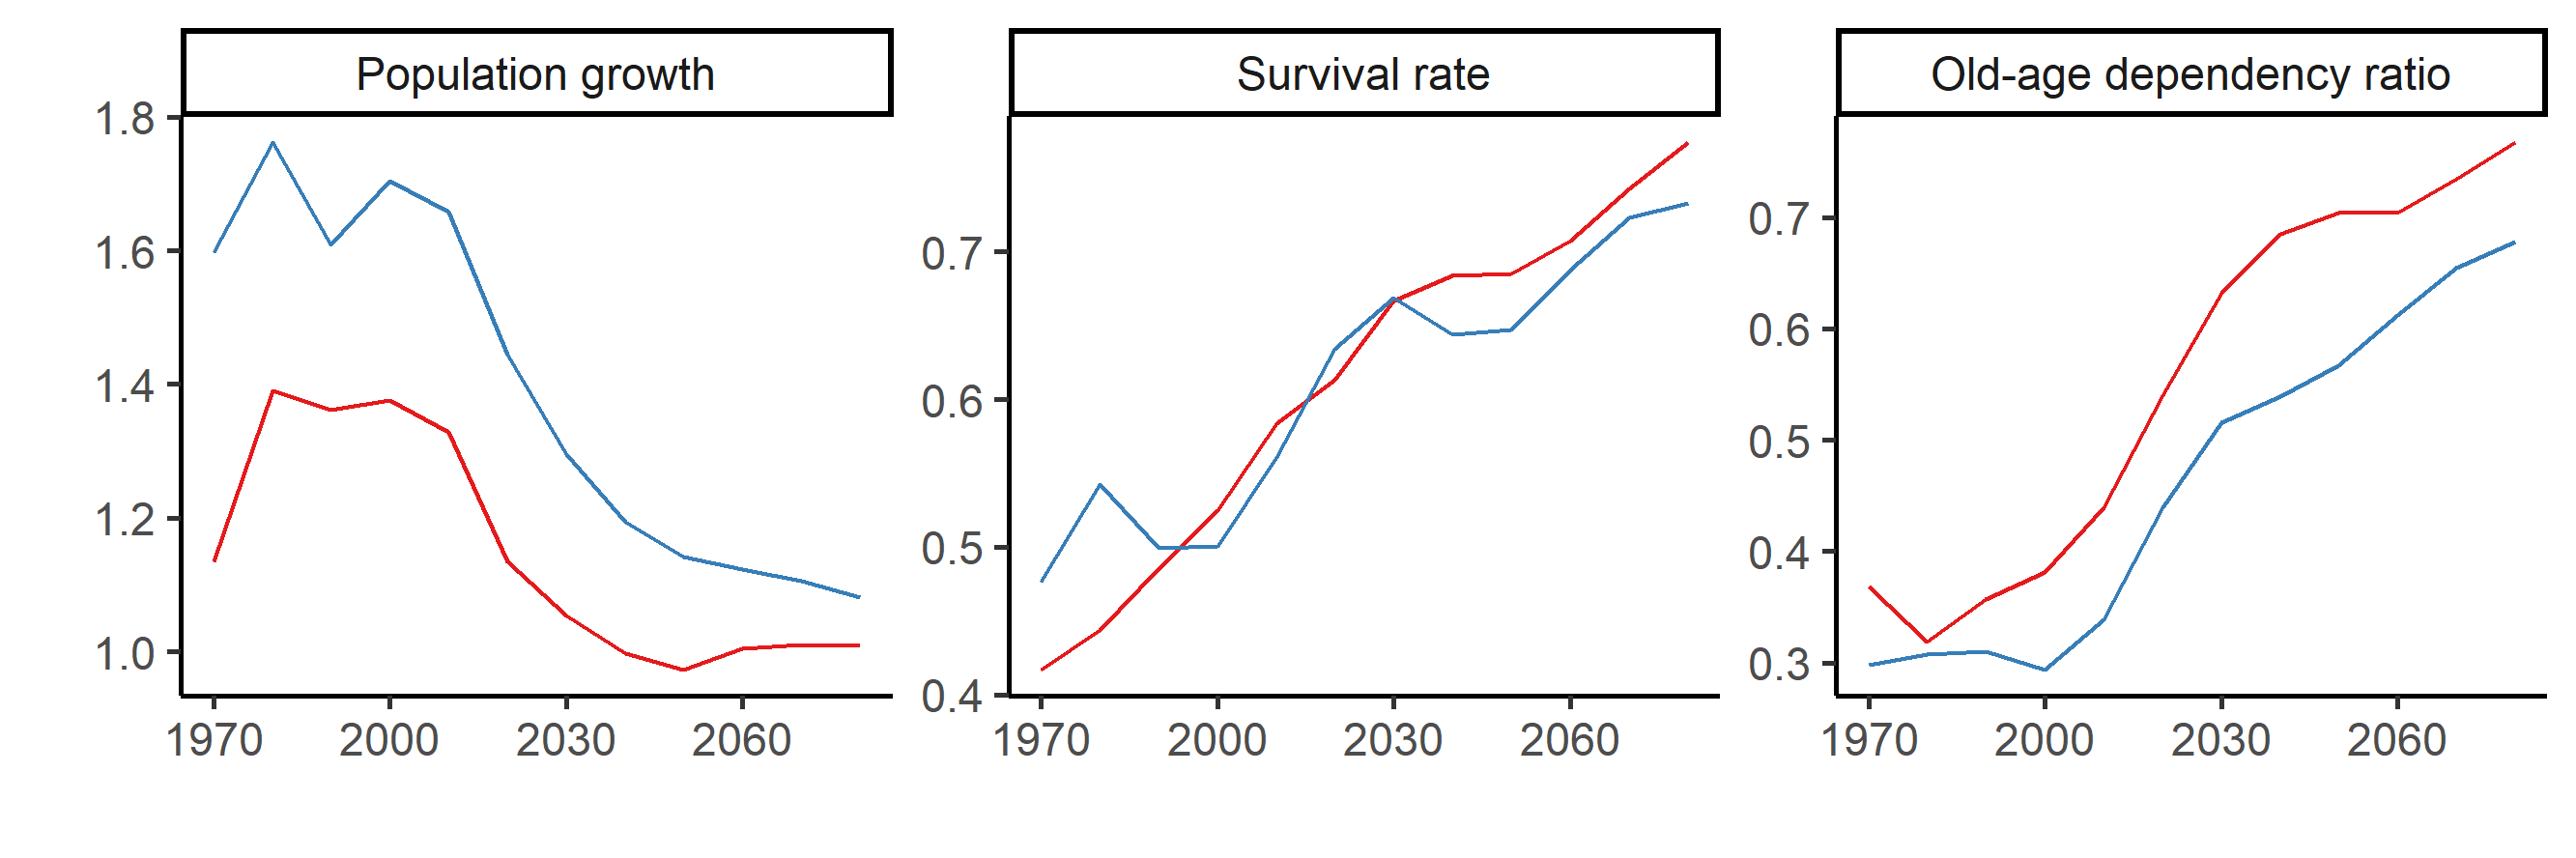
\includegraphics[width=\linewidth]{../result/demo_npdep.png} 
	\caption{Demographic variables time series}\label{fig:demo}
	\vspace{.5ex}
	\hrule
	\vspace{-4ex}
	\justify\singlespacing\footnotesize \textit{Notes:} The black curves refer to France and the gray ones to the United-States.
\end{figure}

%% Normalization %%
Economic variables data ($K_t$, $emp_t$, $Y_t$, $\theta_t$) are taken from the \href{https://www.rug.nl/ggdc/productivity/pwt/}{Penn World Table 9.1}.\footnote{$K$ is the capital stock at constant 2011 national prices, $emp$ the number of persons engaged, $Y$ the real GDP at constant 2011 national prices and $\theta$ the share of labor compensation in GDP. $K$ and $Y$ are adjusted with the average annual hours worked by persons engaged. For further details the reader is referred to \cite{Feenstra2015}.} 
When considering data on the labor share, \cite{Gollin2002} shows that it is necessary to take into account self-employed income. In the model, workers are only young individuals and provide only labor supply. Therefore, I assume that self-employed people earn an income that is characterized as a compensation.\footnote{This specification corresponds to the first adjustment method of \cite{Feenstra2015}.}
I also use the government revenue in \% of GDP from the \href{https://data.oecd.org/tax/tax-revenue.htm}{OECD database} as proxy for the tax rate $\tau_t$.
% Unemployment and redistribution
In the model, labor supply is inelastic and there is no distinction between unemployed and inactive households. Unemployed agents in terms of the model specification corresponds to all agents that do not work. However, in high-income countries, such as France and United States, inactive individuals also benefits from redistribution. This redistribution is captured through unemployment benefits $b_t$ in the model.
I compute the unemployment rate such that $u_t = 1 - emp_t/N^{15-64}_t$, where $N_t^{15-64}$ is the working age population.\footnote{I consider the whole working age population instead of the young population in order to compute the unemployment rate. Due to demographic specification of the model, young agents correspond to those between 20 and 60 years old. The number of persons engaged ($emp$) per age groups are not available in \href{https://www.rug.nl/ggdc/productivity/pwt/}{PWT 9.1}. Therefore, taking only $N^y_t$ as denominator would bias downward the unemployment rate.} Results are robust to different specifications of the unemployment rate.
%\textbf{details in the Appendix (to be written)}. 
Then, I compute labor such that $L_t=(1-u_t)N_t^y$. I normalize $K_t$ and $L_t$ to their 1970 values. As a consequence, the capital-to-labor ratio $k_t$ is also normalized and is equal to 1 in 1970. Then, $N_t^y$ and $N_t^o$ are normalized such that $u_t$ matches the data in 1970.

%% sigma estimation %% %% Parameters to calibrate %%
Once all stock variables are normalized, I calibrate the 7 parameters $\lbrace \phi, \sigma, \gamma, \alpha, \omega, \beta, A \rbrace$. Table \ref{tab:param} summarizes parameters for both countries.
% Parameters table
\begin{table}[tb]
	\caption{Parameters}\label{tab:param}
	\centering
	\begin{threeparttable}
		\begin{tabular}{c l D{.}{.}{-3} D{.}{.}{-3}}
			\multicolumn{2}{c}{\textbf{Parameter}} & \multicolumn{1}{r}{\textbf{France}} & \multicolumn{1}{r}{\textbf{United States}}            \\ \hline \hline
			$\phi$             & Capital share in 1970                           & 0.27 & 0.325		\\ \hline
			$\gamma$           & Relative bargaining power of the union          & 0.5 & 0.5				\\ [-1ex]
			$\alpha$           & Discount rate                                   & 0.669 & 0.669		\\ \hline
			$\sigma$           & Capital-labor elasticity of substitution        & 1.279 & 1.234	\\ \hline
			$\omega$           & Relative ideological spread-out				 & 0.983 & 1.533		\\ [-1ex]
			$\beta$            & Preference for government health expenditure    & 0.739 & 0.138		\\ [-1ex]
			$A$                & Scale parameter of the production function		 & 28.23 & 22.84				\\ \hline \hline
		\end{tabular}
		\vspace{-3ex}
		\begin{tablenotes}
			{\singlespacing\footnotesize
				\item \textit{Note :} Single-equation estimation of $\sigma$ from the two first-order conditions of the profit maximization with normalized CES production function. $\sigma$ estimates are significant at $p<0.1$ for France and $p<0.05$ for the United States. Details in \hyperref[appendix:sigma]{appendix C}.
			}
		\end{tablenotes}
	\end{threeparttable}
\end{table}
The first parameter $\phi$ corresponds to the capital share in 1970. Because the capital-to-labor ratio is normalized (i.e. $k_{1970} = 1$), the labor share $\theta$ in 1970 is equal to $1-\phi$. The main parameter of the model is the elasticity of substitution between capital and labor $\sigma$. I estimate it using a combination of the first order conditions of the profit maximization. Details of the estimation in \hyperref[appendix:sigma]{appendix C}. I obtain 1.279 and 1.234, respectively, for France and the United States. According to the estimation, both input factors are gross substitute. These estimates are in line with \cite{Karabarbounis2014} who use cross-sectional data on 50 countries over the period 1975-2012 to find an elasticity greater than 1 and on average around 1.28 in their baseline estimates. I set the relative bargaining power of the union $\gamma$ to 0.5. Hence, I assume that neither the representative union nor the representative firm have any other advantage in the bargaining apart from their respective outside options. I also set the discount rate at 0.669 according to the literature. Then, I have three remaining parameters that are deduced. The relative ideological spread-out $\omega$ is set such that the model prediction matches the capital-to-labor ratio $k$ in 1970. The preference for government health expenditure $\beta$ is set to match the tax rate $\tau$ in 1970. Finally, the scale parameter of the production function $A$ is set with grid-search to match the average labor share between 2008 and 2012.

Due to initial labor share values, the parameter distribution $\phi$ which correspond to the capital share in 1970 is larger in the United States than in France. Moreover, the relative per-capita political influence of old households $\omega$ is also greater. This deduced parameter suggests that young generations have less political weight in the United States compared to France. Notice that $\omega$ is lower than one for France. It implies that French youth voting behavior is more sensitive to policy changes compared to elderly. French households have a much greater preference for government health expenditure $\beta$. Finally, the scale parameter $A$ is ranged between 20 and 30 for both countries.

\subsection{Model predictions over the period 1970-2010}\label{subsec:model_pred}

\subsubsection{The labor share decline}

Figure \ref{fig:baseline7010} displays the labor share from model predictions and data over the period 1970-2010.
\begin{figure}[tb]
	\centering
	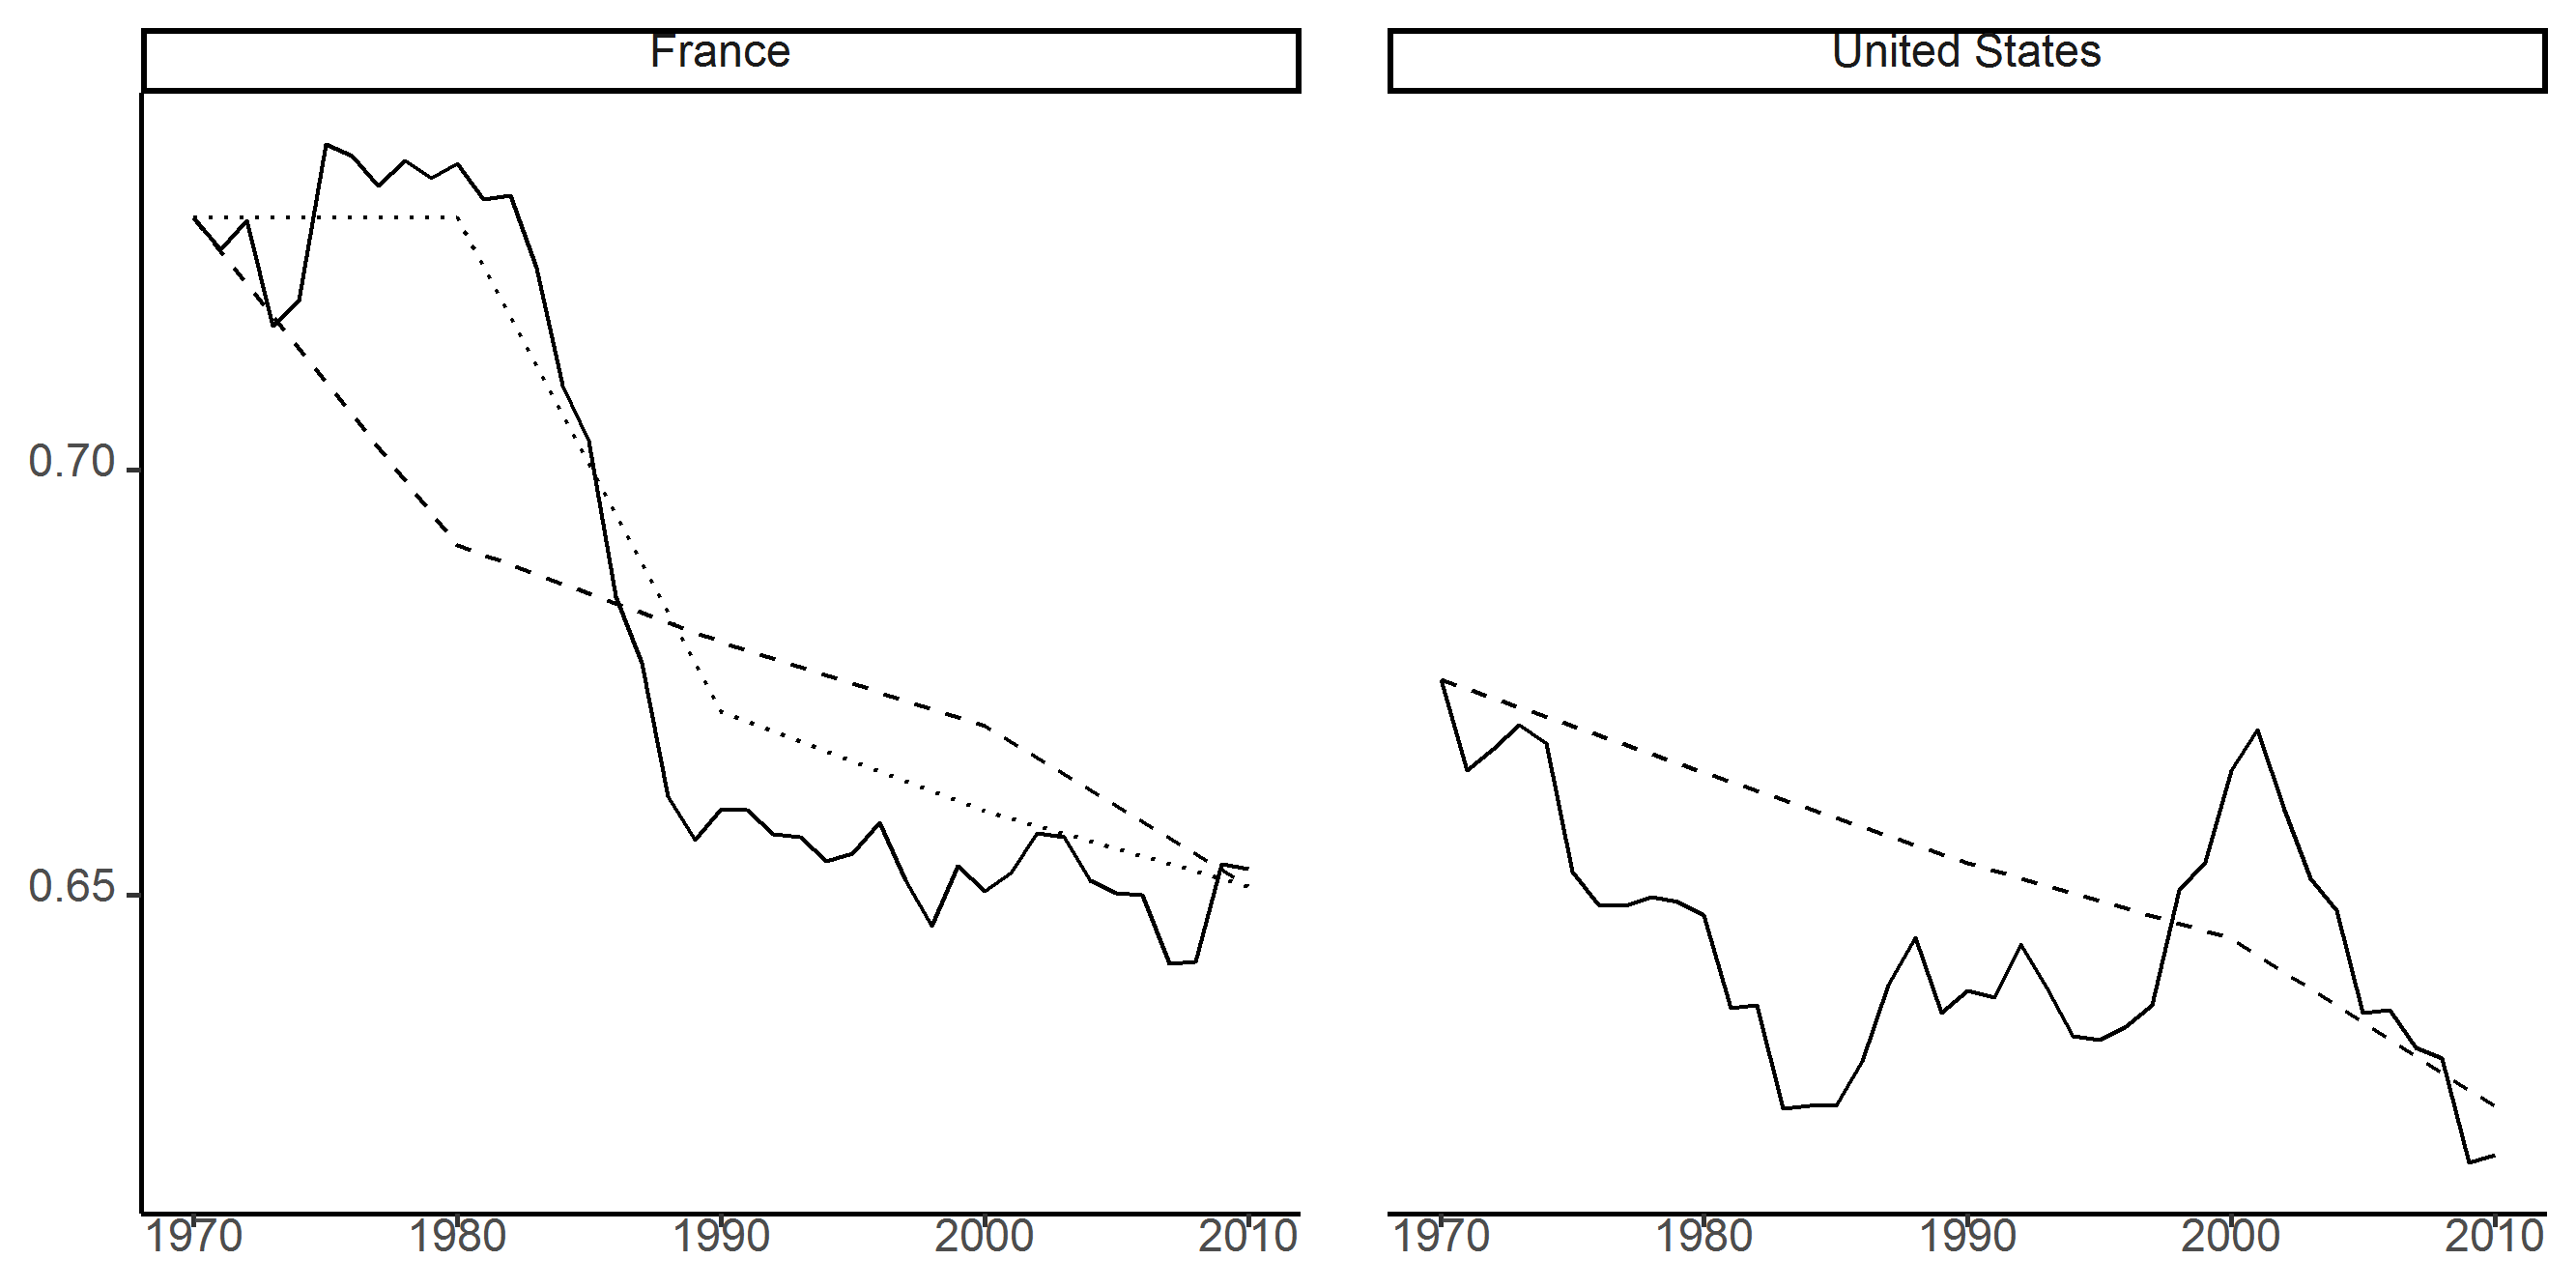
\includegraphics[width=1\linewidth]{../result/baseline7010.png}
	\caption{Model prediction of the labor share}
	\label{fig:baseline7010}
	\vspace{.5ex}
	\hrule
	\vspace{-4ex}
	\justify\singlespacing\footnotesize \textit{Notes:} The solid curve corresponds to the labor share in the data, from the \href{https://www.rug.nl/ggdc/productivity/pwt/}{Penn World Table 9.1} with adjustment method 1. The dashed curve is the model prediction with a unique capital-labor elasticity of substitution. The dotted curve is the model prediction for France with a break in the regime for the capital-labor elasticity of substitution (details in \hyperref[appendix:regime]{appendix D}).
\end{figure}
The model reproduces the global trend of the data for both countries. For France, the model is not able to reproduce the huge decline of the labor share between 1980 and 1990. This gap may be explained by different factors not considered in the model.
%% Firing cost : Bentolila and Bertola
I modelize the workers outside option within the wage bargaining using only unemployment benefits and the tax rate. Other labor market institutions may have played a role in firms' employment policies during this period. Indeed, I consider a right-to-manage specification, meaning that the firm has the prerogative to hire and fire. In my framework, there is no firing cost. \cite{Bentolila1990} build a model with linear adjustment cost and find that firing costs have an effect on firms propensity to hire and fire. Further, they also find that firing costs slightly increase average long-run employment. Subsequent to the oil shock, firms were not able to fire as they would have due to high firing costs.\footnote{\cite{Blanchard1997} also shows that wages failed to adjust to the productivity slowdown and adverse supply shocks of the 1970s. Thus, wages remained relatively high and so did the labor share. This phenomenon was more pronounced in European Continental countries than in the Anglo-Saxon countries, mainly due to labor market institutions.} They reduced employment with attrition, thus the process took time and the employment remained higher than it should during some years. In addition, most of the employment security policies were introduced between the 1960s and the beginning of the 1970s. Here again, these protections may be the result of the baby-boomers generation operating a political pressure to secure employment. Although, I do not integrate it in the model. Then, France during the 1980s has started to implement policies in order to make the labor market more flexible. For instance, short term contracts have been introduced in 1979. To summarize, the labor market institutions in France were tremendously different before and after the 1980s. The reason why the model prediction does not reproduce the labor share from the data owes to the calibration of the model that is in line with the labor market institutions after 1980, but not before. Another way to think about it, in terms of the model, is to suppose that the capital-labor elasticity of substitution was much smaller before 1980.\footnote{Perhaps even lower than 1, meaning that an increase in $k_t$ leads to an increase in $\theta_t$.} Therefore, the representative firm was constrained and not able to substitute labor by capital as much as the model predicts.
%% Other reason ?
%\textbf{Blanchard ? / Outside option ?}.
In line with the above arguments, I investigate whether there is a change in the regime of $\sigma$ over this period. Details of the methodology in \hyperref[appendix:regime]{appendix D}. I find that such a break has occurred during the 1980s in France. The dotted curve is the model prediction with a capital-labor elasticity of substitution of 1 in 1970-1980 and about 1.321 thereafter. The scale parameter $A$ is also changed to 23.891 for France.
For the United States, the model tends to overestimate the labor share in 1980 and 1990 and underestimate it in 2000.
%\textbf{Explanations / References ?}. 
However, model predictions capture the global trend of the labor share over the period.
%% Transition Mechanism analysis
To highlight the mechanisms of this decline, it is necessary to look at the variations of determinant variables.

\subsubsection{Mechanisms of the decline}

The state of the economy is determined by the interaction of the wage bargaining and the voting. Both processes take place simultaneously. The demographic context over this period, as presented in figure \ref{fig:demo}, is such as the population growth $n_t$ slightly exceeds the increasing survival rate $p_t$. Thus, the old-age-dependency $p_t/n_t$ remains relatively constant between 1970 and 2000. With a decline in France in 1980 due to the massive entry of the baby-boomers in the labor force. Finally, the old-age-dependency ratio starts to increase between 2000 and 2010 due to a steady population growth but a sharply increasing survival rate. This increase is also due to the baby-boomers' cohort who begins to retire. As a result of this demographic context, the youth political weight $\eta_t$ was above its 1970's level until 2000 in both countries.

% Public Policy
Figure \ref{fig:dev_public7010} displays the deviation from the 1970 steady-state of public policy variables in percentage.
\begin{figure}[tb]
	\centering
	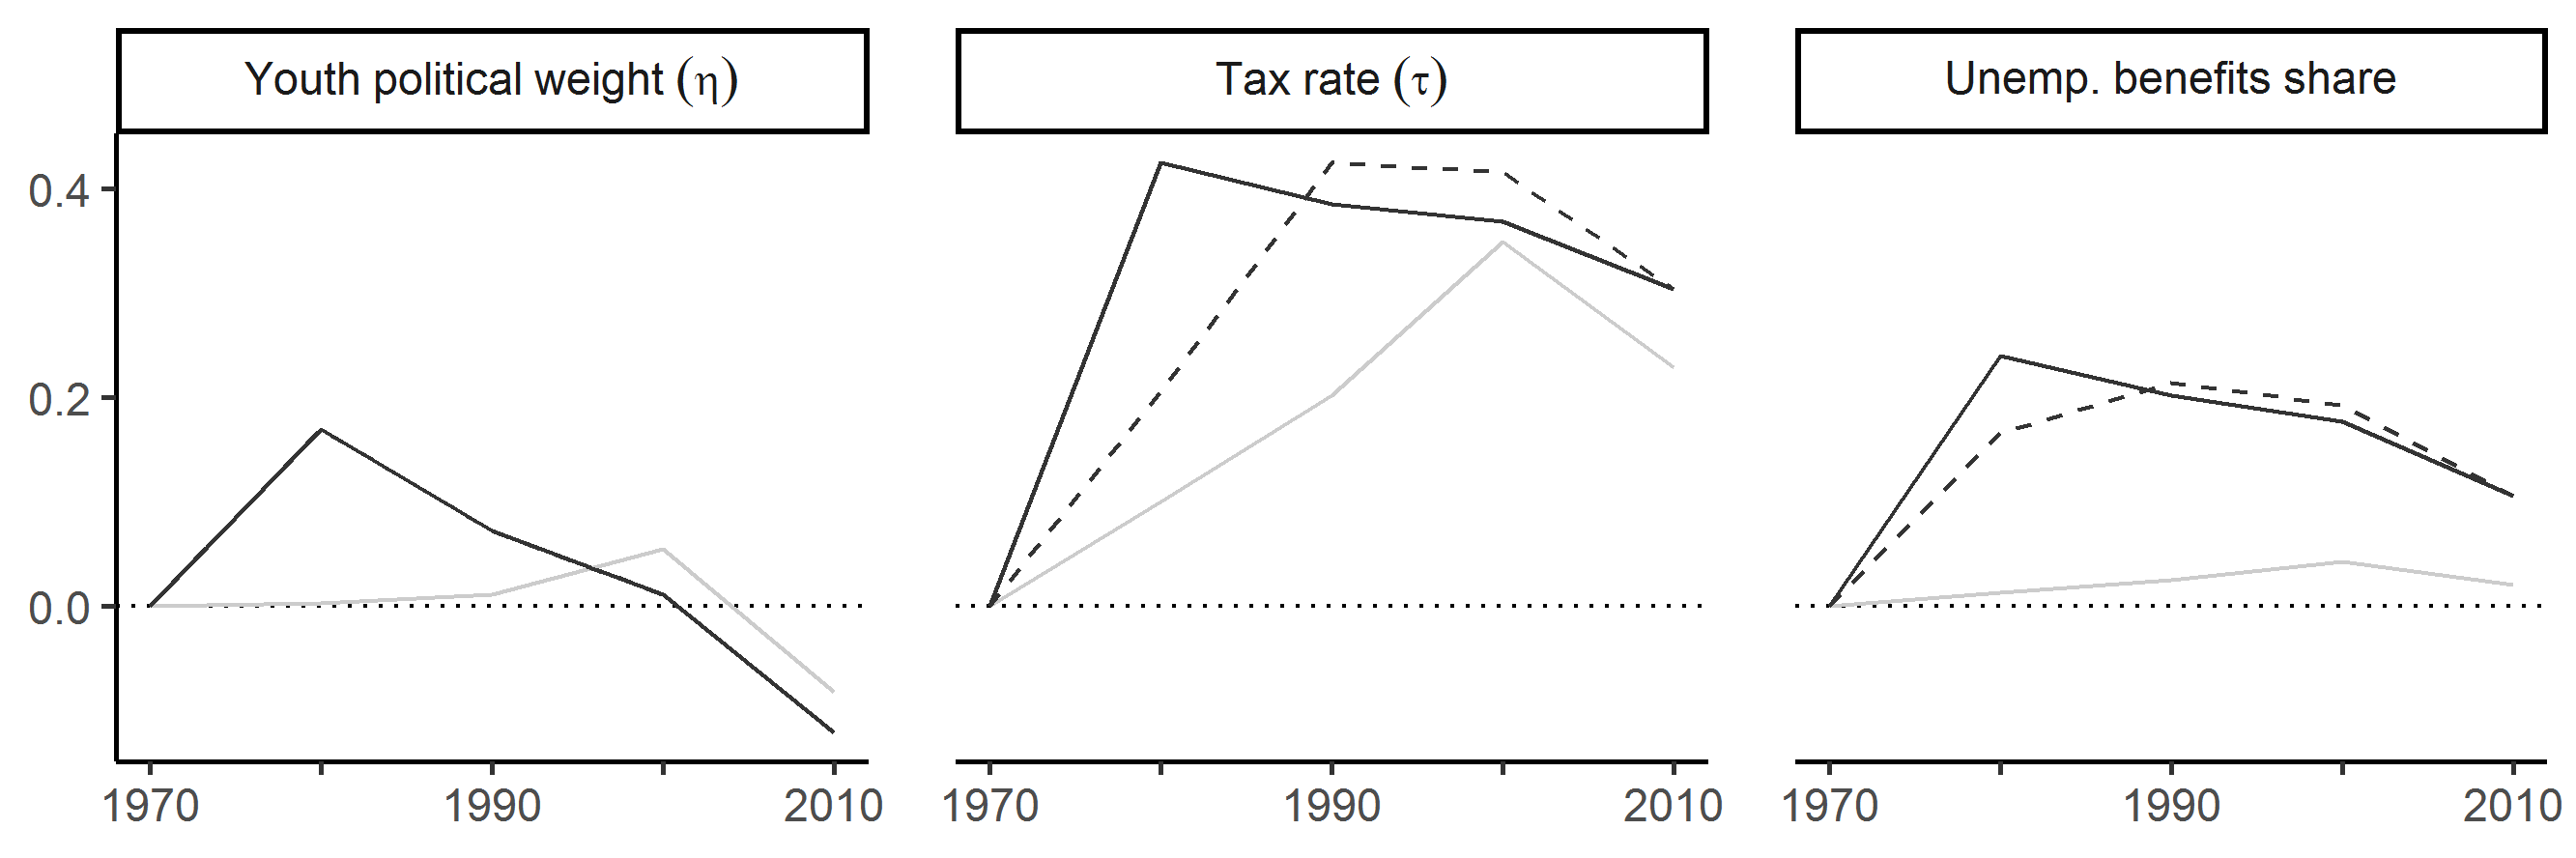
\includegraphics[width=1\linewidth]{../result/deviation/dev_public7010.png}
	\caption{Deviation from the 1970 steady-state of public policy variables}
	\label{fig:dev_public7010}
	\vspace{.5ex}
	\hrule
	\vspace{-4ex}
 	\justify\singlespacing\footnotesize \textit{Notes:} The unemp. benefits share corresponds to the share of the unemployment benefits in the government spending, i.e. $buN^y/(\tau Y)$. The black curves refer to France and the gray ones to the United-States. The solid curves refer to the model predictions with a unique capital-labor elasticity of substitution and the dashed ones to the model prediction for France with a break in the regime for the capital-labor elasticity of substitution.
\end{figure}
As the youth political weight raises and because they desire more redistribution, the tax rate $\tau_t$ increases (i.e. $\partial \tau_t / \partial \eta_t > 0$). Due to the opportunistic behavior of political parties, pro-youth policies are implemented. In the model, pro-youth policies correspond to pro-labor policies and are translated in terms of unemployment benefits in order to insure the unemployment risk. Thus, the unemployment benefits share in government revenue $b~share$ increases at the cost of the government health spending share in government revenue.

% Outside option
%Figure \ref{fig:dev_outside_7010} displays the deviation from the 1970 steady-state of outside option variables in percentage.
%\begin{figure}[!ht]
%	\centering
%	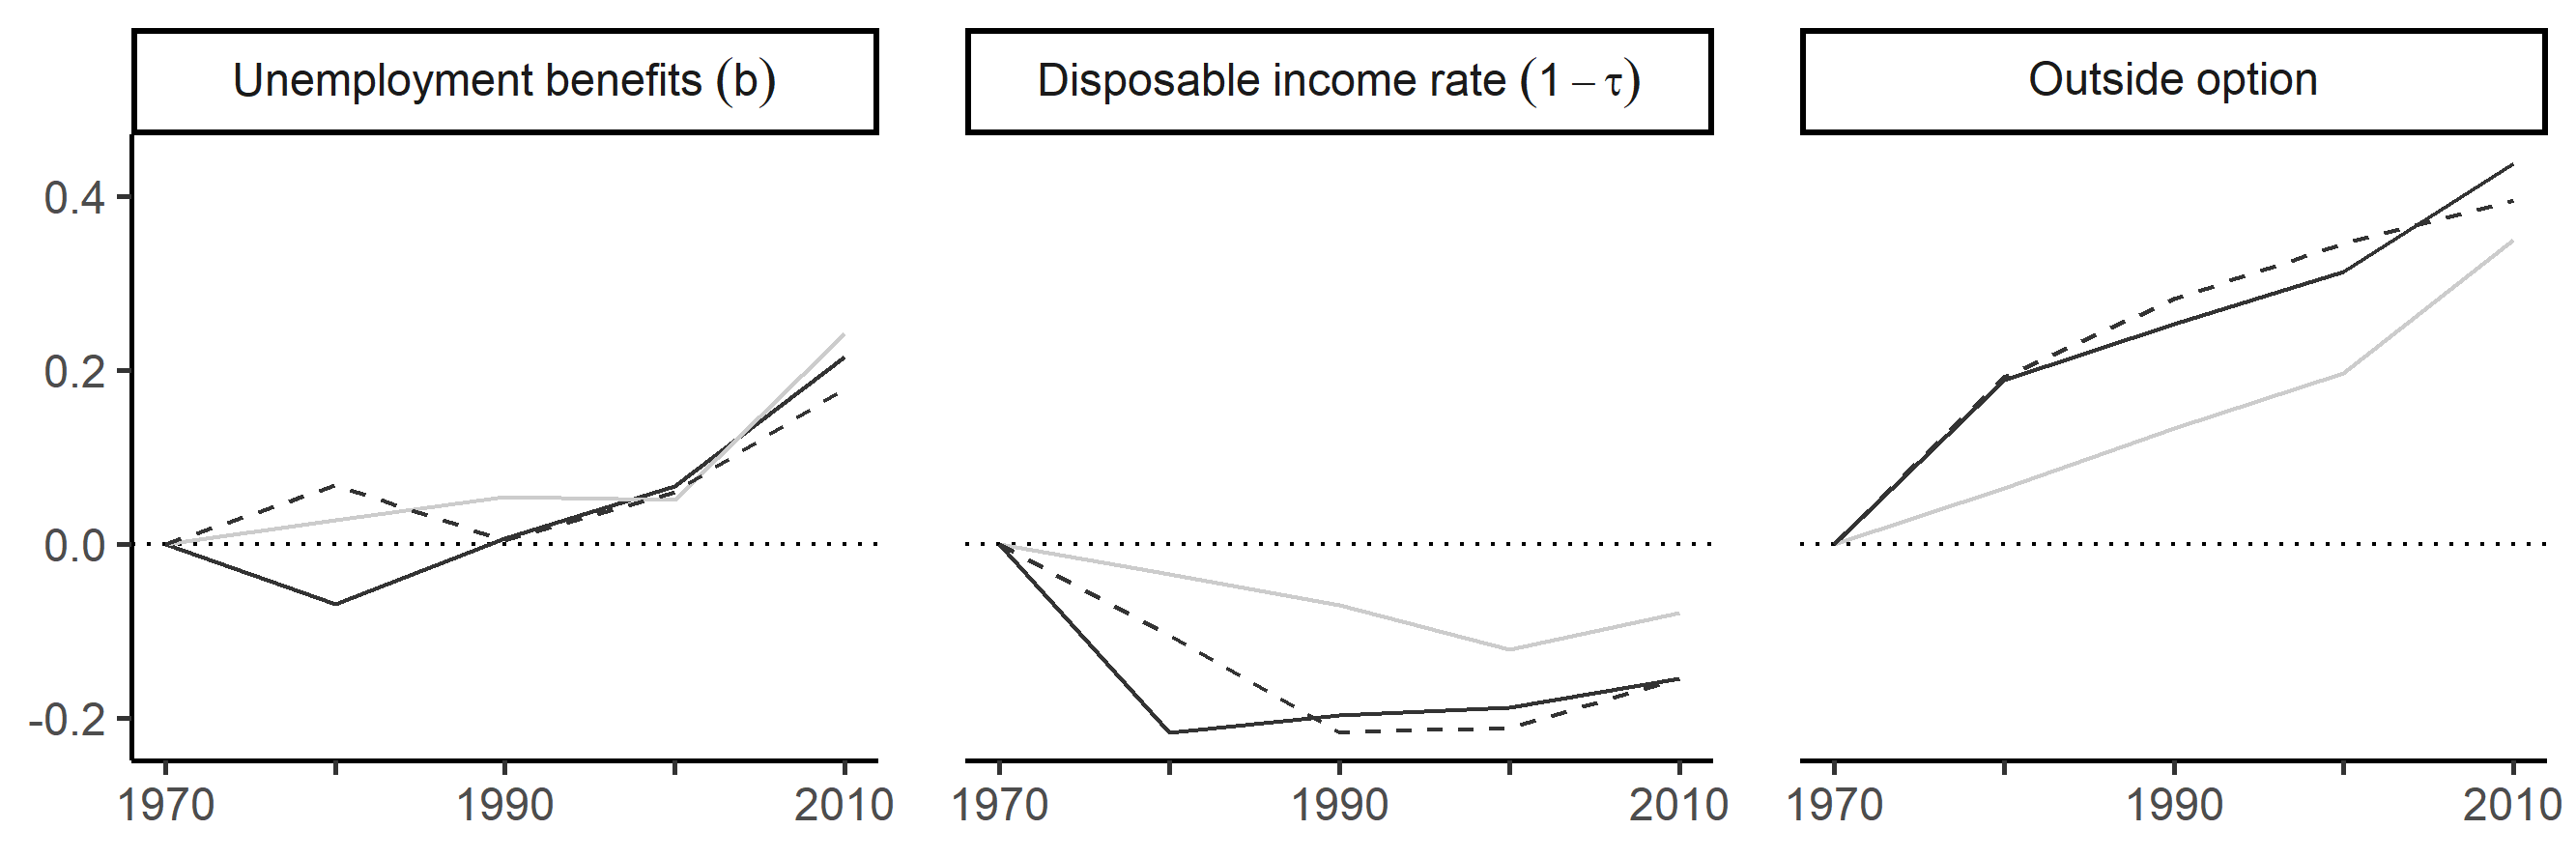
\includegraphics[width=1\linewidth]{../result/deviation/dev_outside7010.png}
%	\caption{Deviation from the 1970 steady-state of outside option variables.}
%	\label{fig:dev_outside_7010}
%	\vspace{.5ex}
%	\hrule
%	\vspace{-4ex}
%	\justify\singlespacing\footnotesize $b$ is the unemployment benefits per capita, $1-\tau$ \textbf{the disposable income rate} and $b/(1-\tau)$ the outside option. The reader is referred to the footnote of the figure \ref{fig:pred_data_7010} for the legend of the curves.
%\end{figure}

% Wage bargaining
These policy changes interact with the wage bargaining because they affect the outside option of the young agents. Figure \ref{fig:dev_bargain7010} displays the deviation from the 1970 steady-state of wage bargaining variables in percentage.
\begin{figure}[tb]
	\centering
	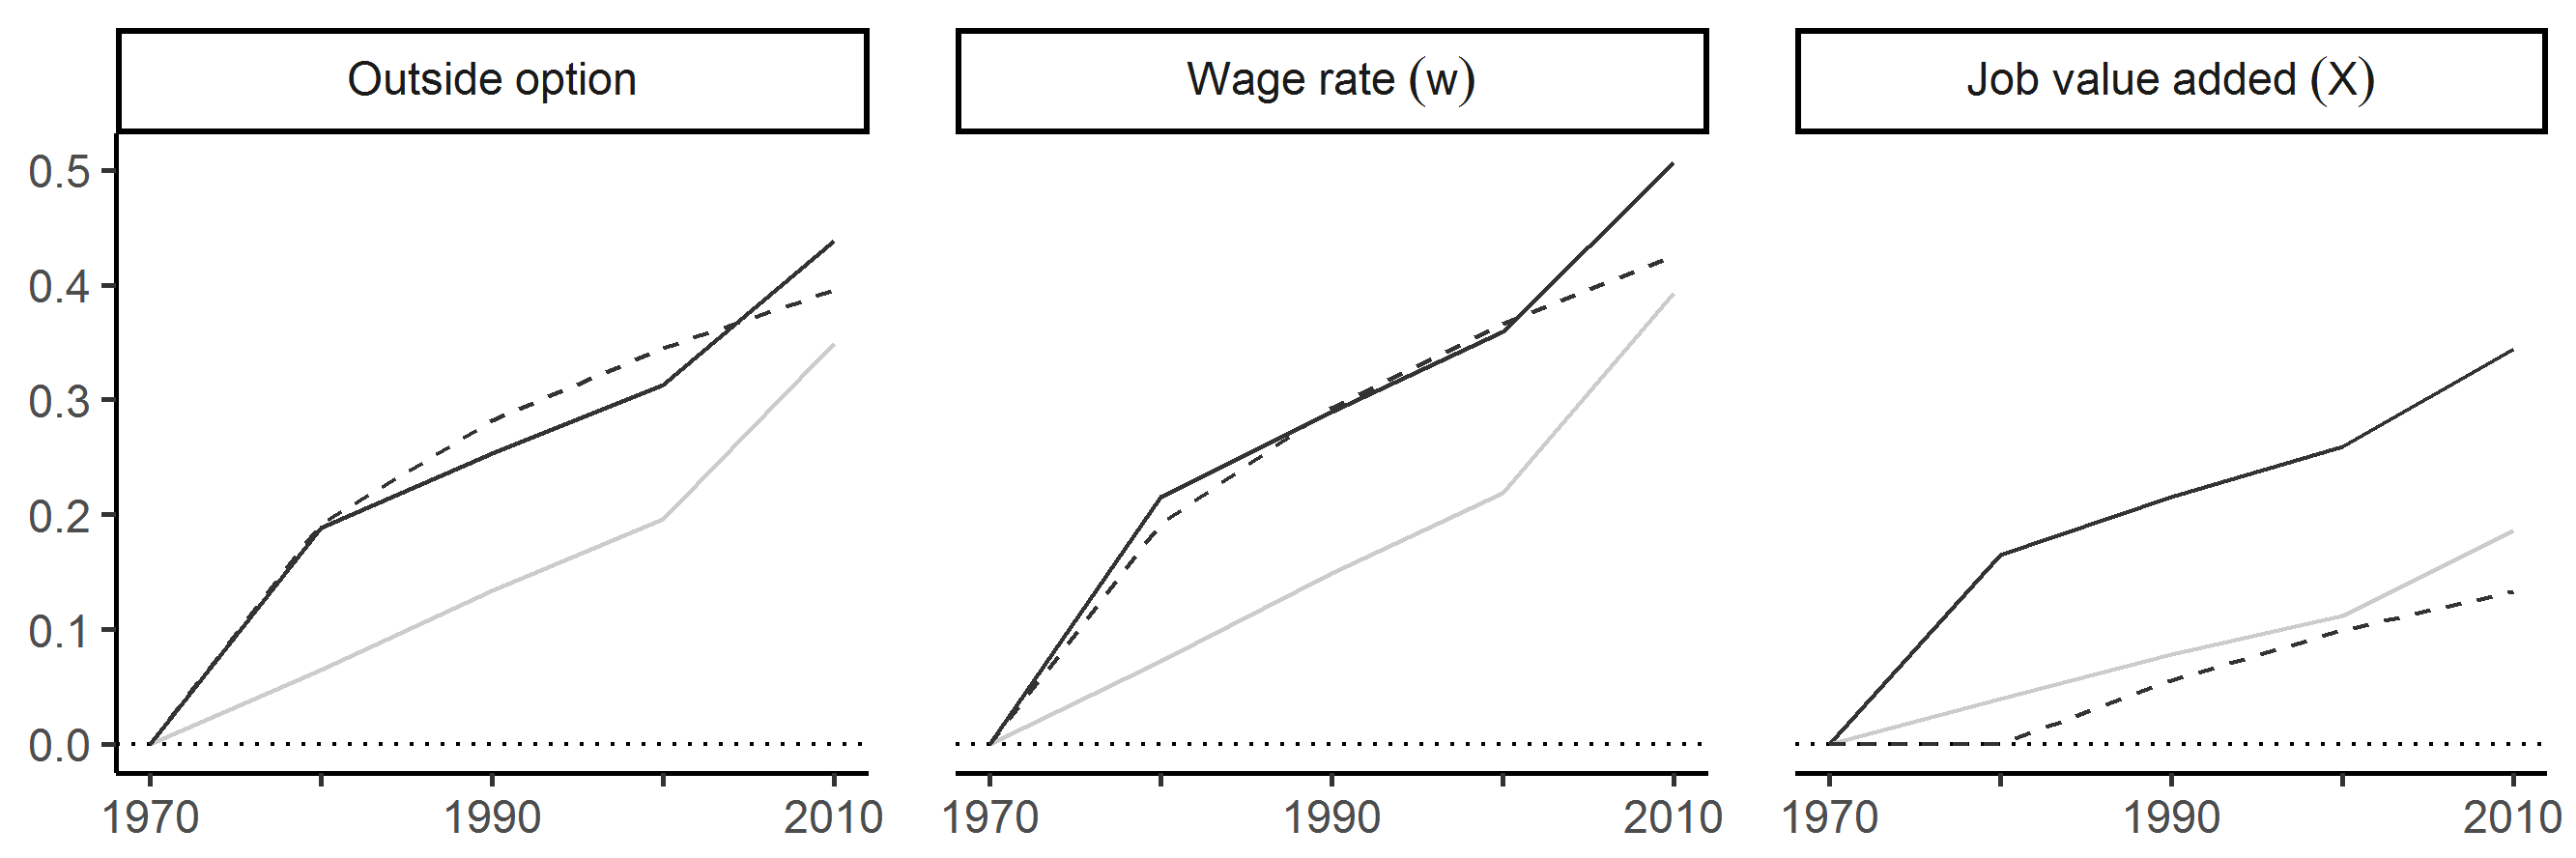
\includegraphics[width=1\linewidth]{../result/deviation/dev_bargain7010.png}
	\caption{Deviation from the 1970 steady-state of wage bargaining variables}
	\label{fig:dev_bargain7010}
	\vspace{.5ex}
	\hrule
	\vspace{-4ex}
	\justify\singlespacing\footnotesize \textit{Notes:} The outside option corresponds to $b/(1-\tau)$. The reader is referred to the footnote of the figure \ref{fig:dev_public7010} for the legend of the curves.
\end{figure}
Pro-youth public policies motivated by a higher youth political weight leads to an increase of the unemployment benefits and a decline of the disposable income rate $(1-\tau_t)$. These two variables determine the outside option $b_t/(1-\tau_t)$ within the wage bargaining. The decrease of the denominator exceeds the increase of the numerator. Thus, the net effect on the outside option is positive and allows workers to bargain a greater wage $w_t$. The gain in net wage $(1-\tau_t)w_t$ exceeds the one in unemployment benefits per capita $b_t$. Hence, employment is even more worth as unemployment in terms of utility (i.e. $dX_t > 0$).

% Production
Due to the ability of workers to bargain a greater wage, the representative firm shifts away from labor. Figure \ref{fig:dev_prod7010} displays the deviation from the 1970 steady-state of production function variables in percentage.
\begin{figure}[tb]
	\centering
	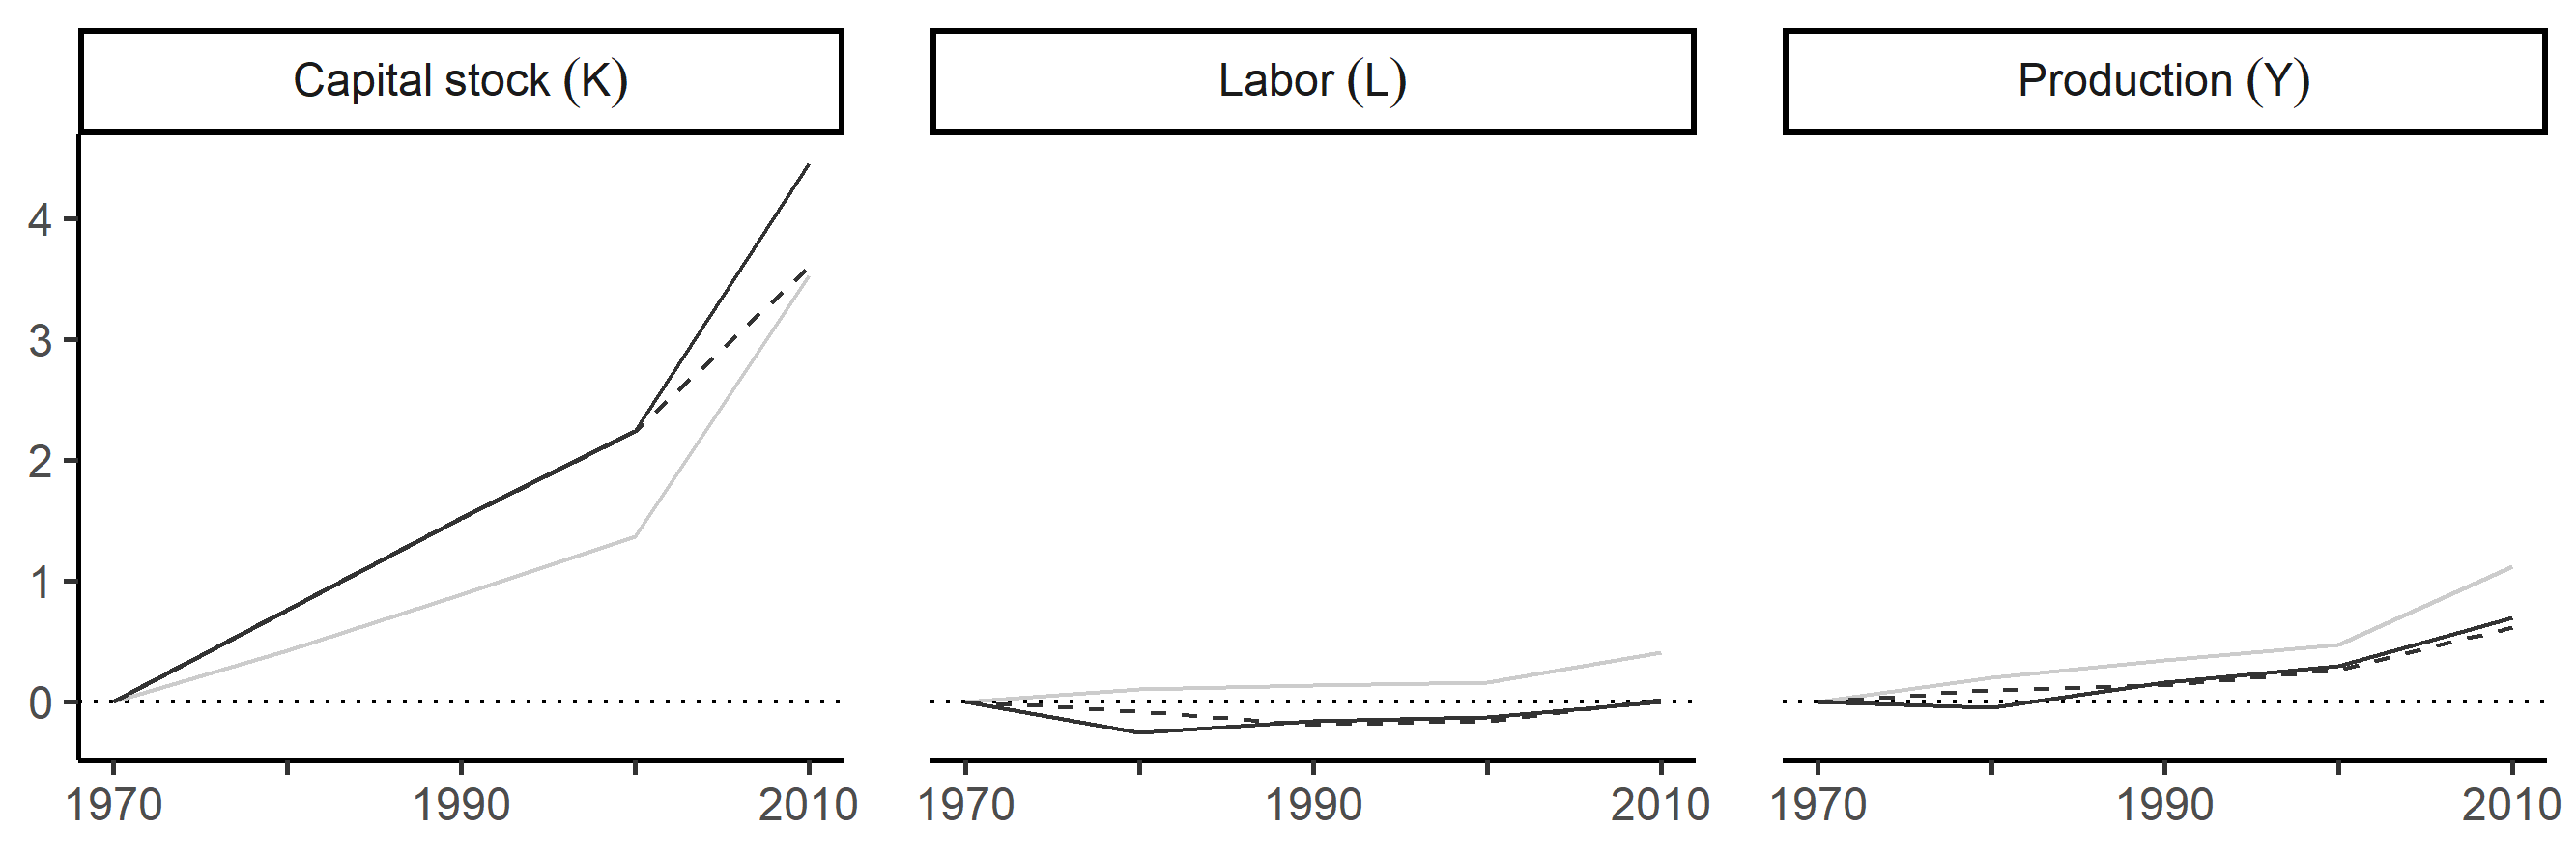
\includegraphics[width=1\linewidth]{../result/deviation/dev_prod7010.png}
	\caption{Deviation from the 1970 steady-state of production function variables}
	\label{fig:dev_prod7010}
	\vspace{.5ex}
	\hrule
	\vspace{-4ex}
	\justify\singlespacing\footnotesize \textit{Notes:} The reader is referred to the footnote of the figure \ref{fig:dev_public7010} for the legend of the curves.
\end{figure}
This behavior is permitted by two features of the model. First, the right-to-manage specification of the wage bargaining enables the firm to hire and fire as much as wanted. Second, the capital-labor elasticity of substitution $\sigma$ is greater than unity for both countries. Thus, both input factors are gross substitute. The firm is able to substitute labor with capital for a given output level. This behavior leads to a decline of the number of worker $L_t$ because the labor cost (i.e. the wage) has increased. Notice that the substitution effect is more vigorous in France because of the relatively higher elasticity of substitution $\sigma$. French firms are able to substitute relatively more labor with capital and also have a faster growth in capital stock $K_t$. Thus, the number of workers becomes lower than its 1970's level in France. While the United-States manage to slightly increase its labor factor. As a consequence, the US production $Y_t$ grows faster.

% Unemployment
The slowdown in employment has consequences on the labor market. Figure \ref{fig:dev_unemp7010} displays the deviation from the 1970 steady-state of unemployment's component variables in percentage.
\begin{figure}[tb]
	\centering
	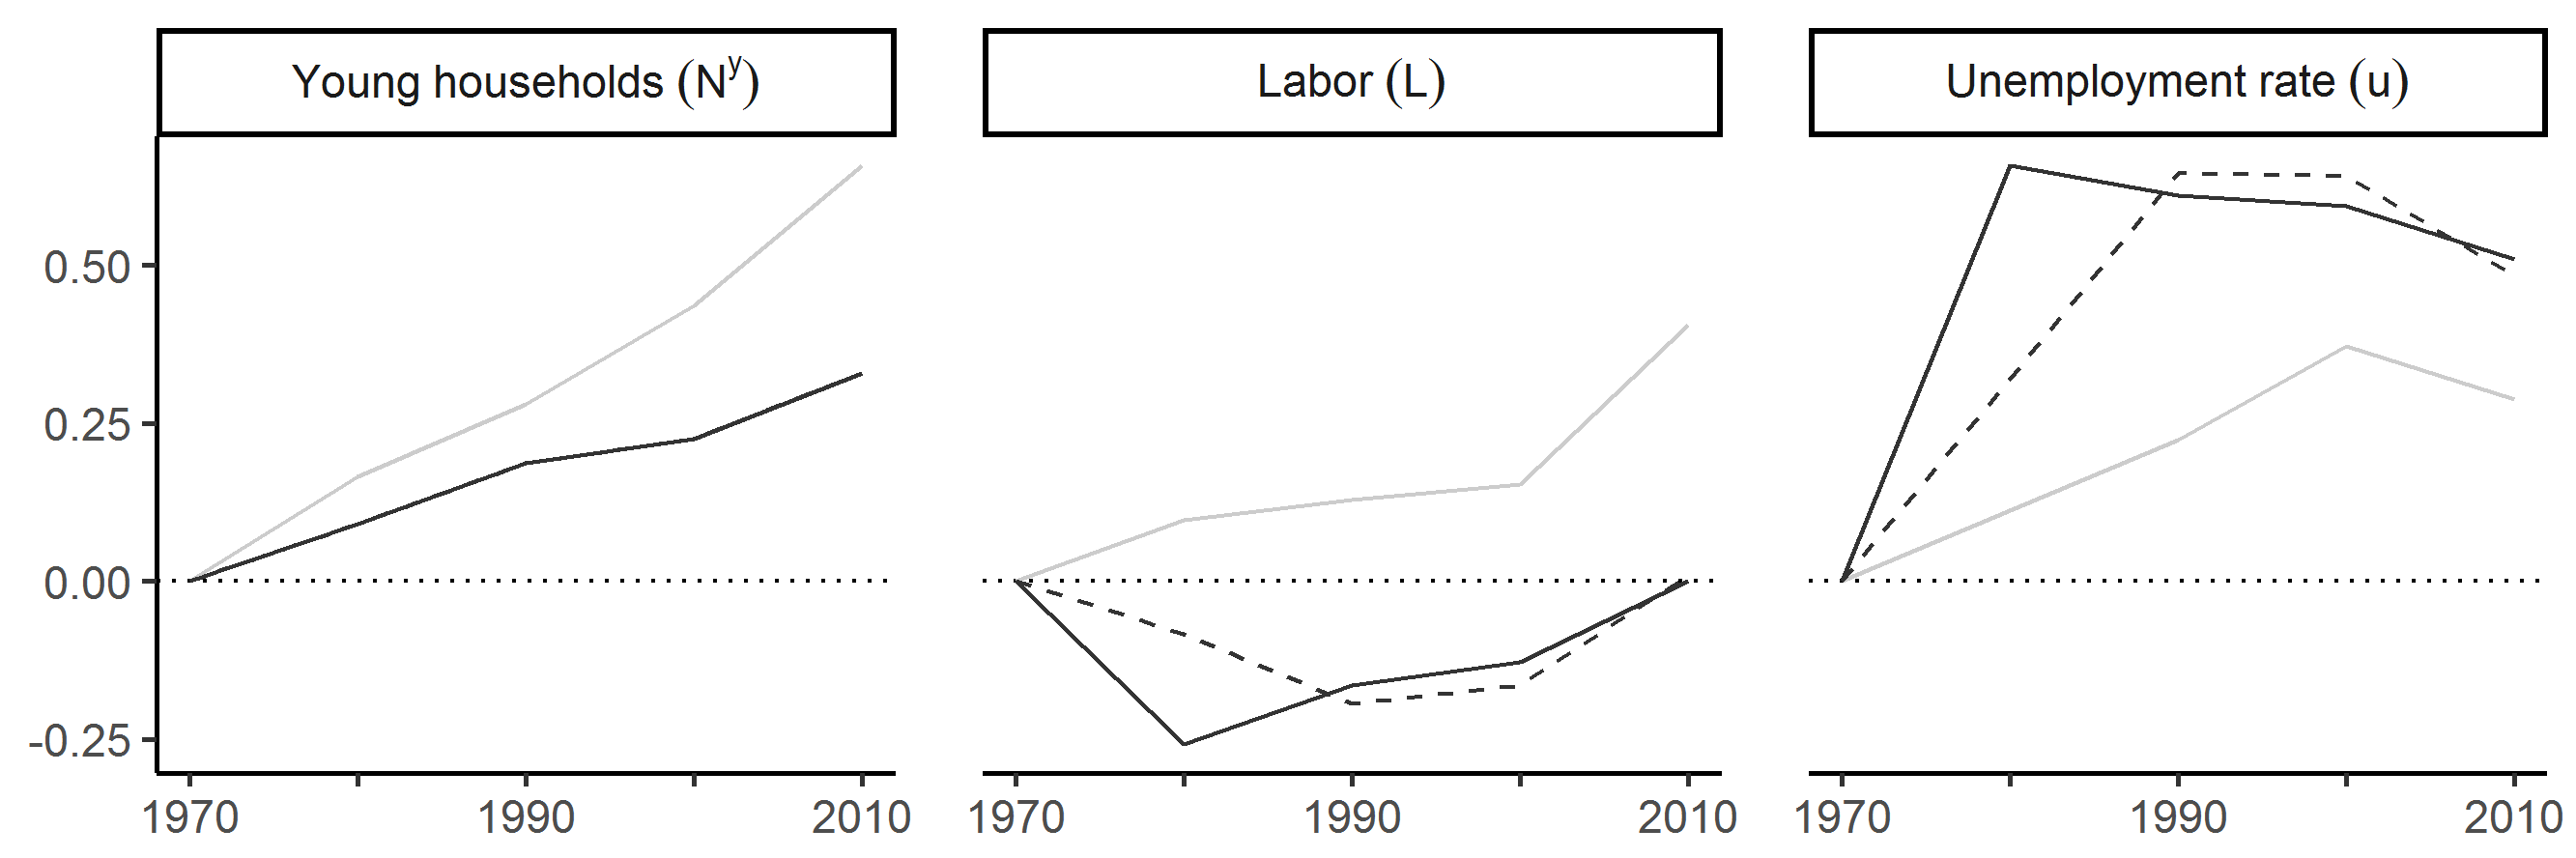
\includegraphics[width=1\linewidth]{../result/deviation/dev_unemp7010.png}
	\caption{Deviation from the 1970 steady-state of unemployment's component variables}
	\label{fig:dev_unemp7010}
	\vspace{.5ex}
	\hrule
	\vspace{-4ex}
	\justify\singlespacing\footnotesize \textit{Notes:} The reader is referred to the footnote of the figure \ref{fig:dev_public7010} for the legend of the curves.
\end{figure}
This slowdown in employment directly raises unemployment in France by reducing the number of workers. Furthermore, the effect is all the more tremendous because the labor force $N_t^y$ grows due to the baby-boomers' arrival. The United-States also know a growing population but the impact on unemployment is much weaker due to the increasing number of workers, as discussed above.

% Labor share components
The dynamics of the production function affects the determinants of the labor share. Figure \ref{fig:dev_laborshare7010} displays the deviation from the 1970 steady-state of labor share's component variables in percentage.
\begin{figure}[tb]
	\centering
	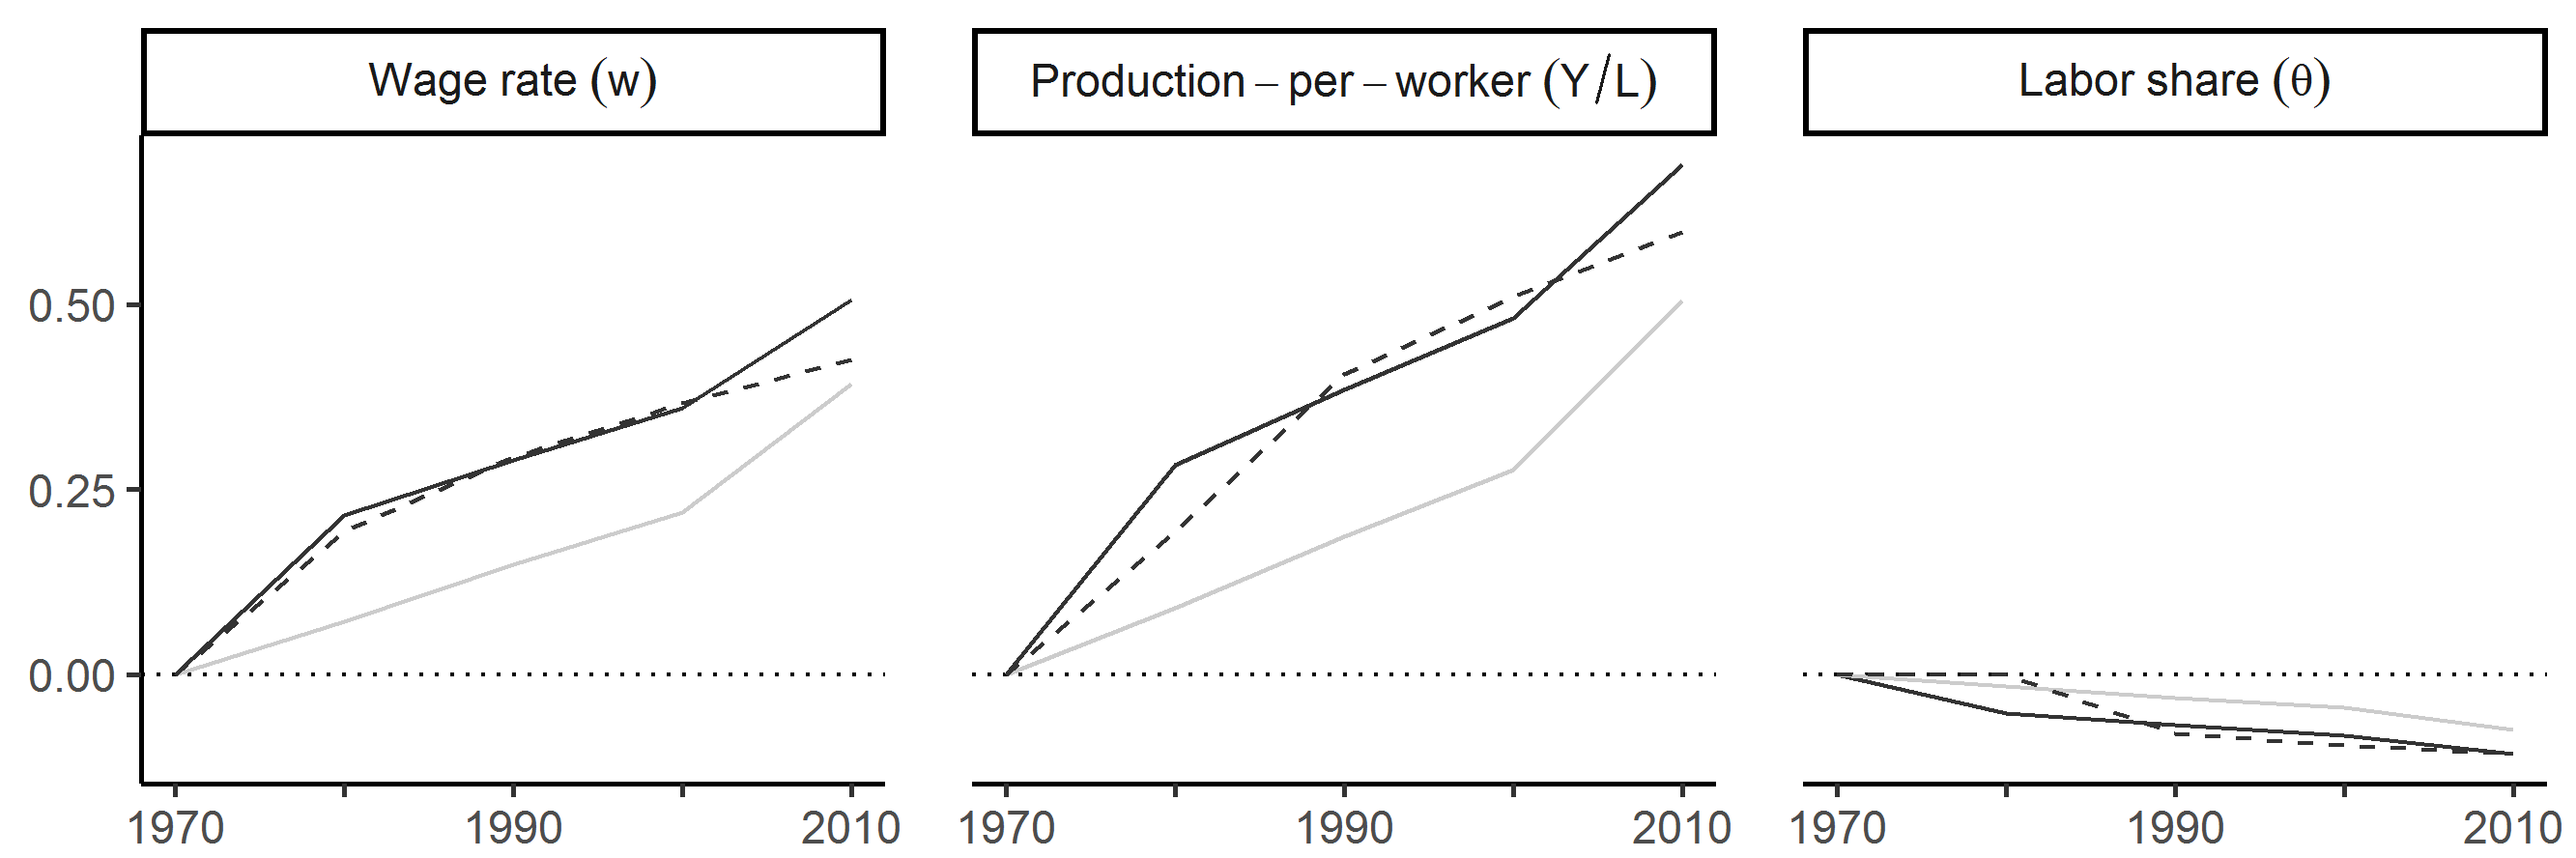
\includegraphics[width=1\linewidth]{../result/deviation/dev_laborshare7010.png}
	\caption{Deviation from the 1970 steady-state of labor share's component variables}
	\label{fig:dev_laborshare7010}
	\vspace{.5ex}
	\hrule
	\vspace{-4ex}
	\justify\singlespacing\footnotesize \textit{Notes:} The reader is referred to the footnote of the figure \ref{fig:dev_public7010} for the legend of the curves.
\end{figure}
Due to the fact that both input factors are gross substitute, the output-per-worker $Y_t/L_t$ increases when the capital-per-worker $k_t$ does so. This increase exceeds the one of the wage. As a result, the labor share declines.

Let summarize the mechanisms over this period. The youth fosters a pro-labor public policy due to a relatively high political weight. This institutional design raises the outside option of the workers. It gives more bargaining power to the union who is able to bargain greater wages. The cost of labor becoming too high, the firms decide to shift away from labor. The fact that both input factors are gross-substitute allows firms to substitute labor with capital. The shift-away from labor engenders an increase of the output-per-worker which thwarts and exceeds the wage gain. Thus, the labor share declines. Moreover, unemployment rises due to a growing labor force.

\subsection{Model predictions over the period 2010-2080}

\subsubsection{The labor share resurgence}

%% Description of the graph
Figure \ref{fig:baseline1080} displays the model predicted labor share over the period 1970-2080.
\begin{figure}[tb]
	\centering
	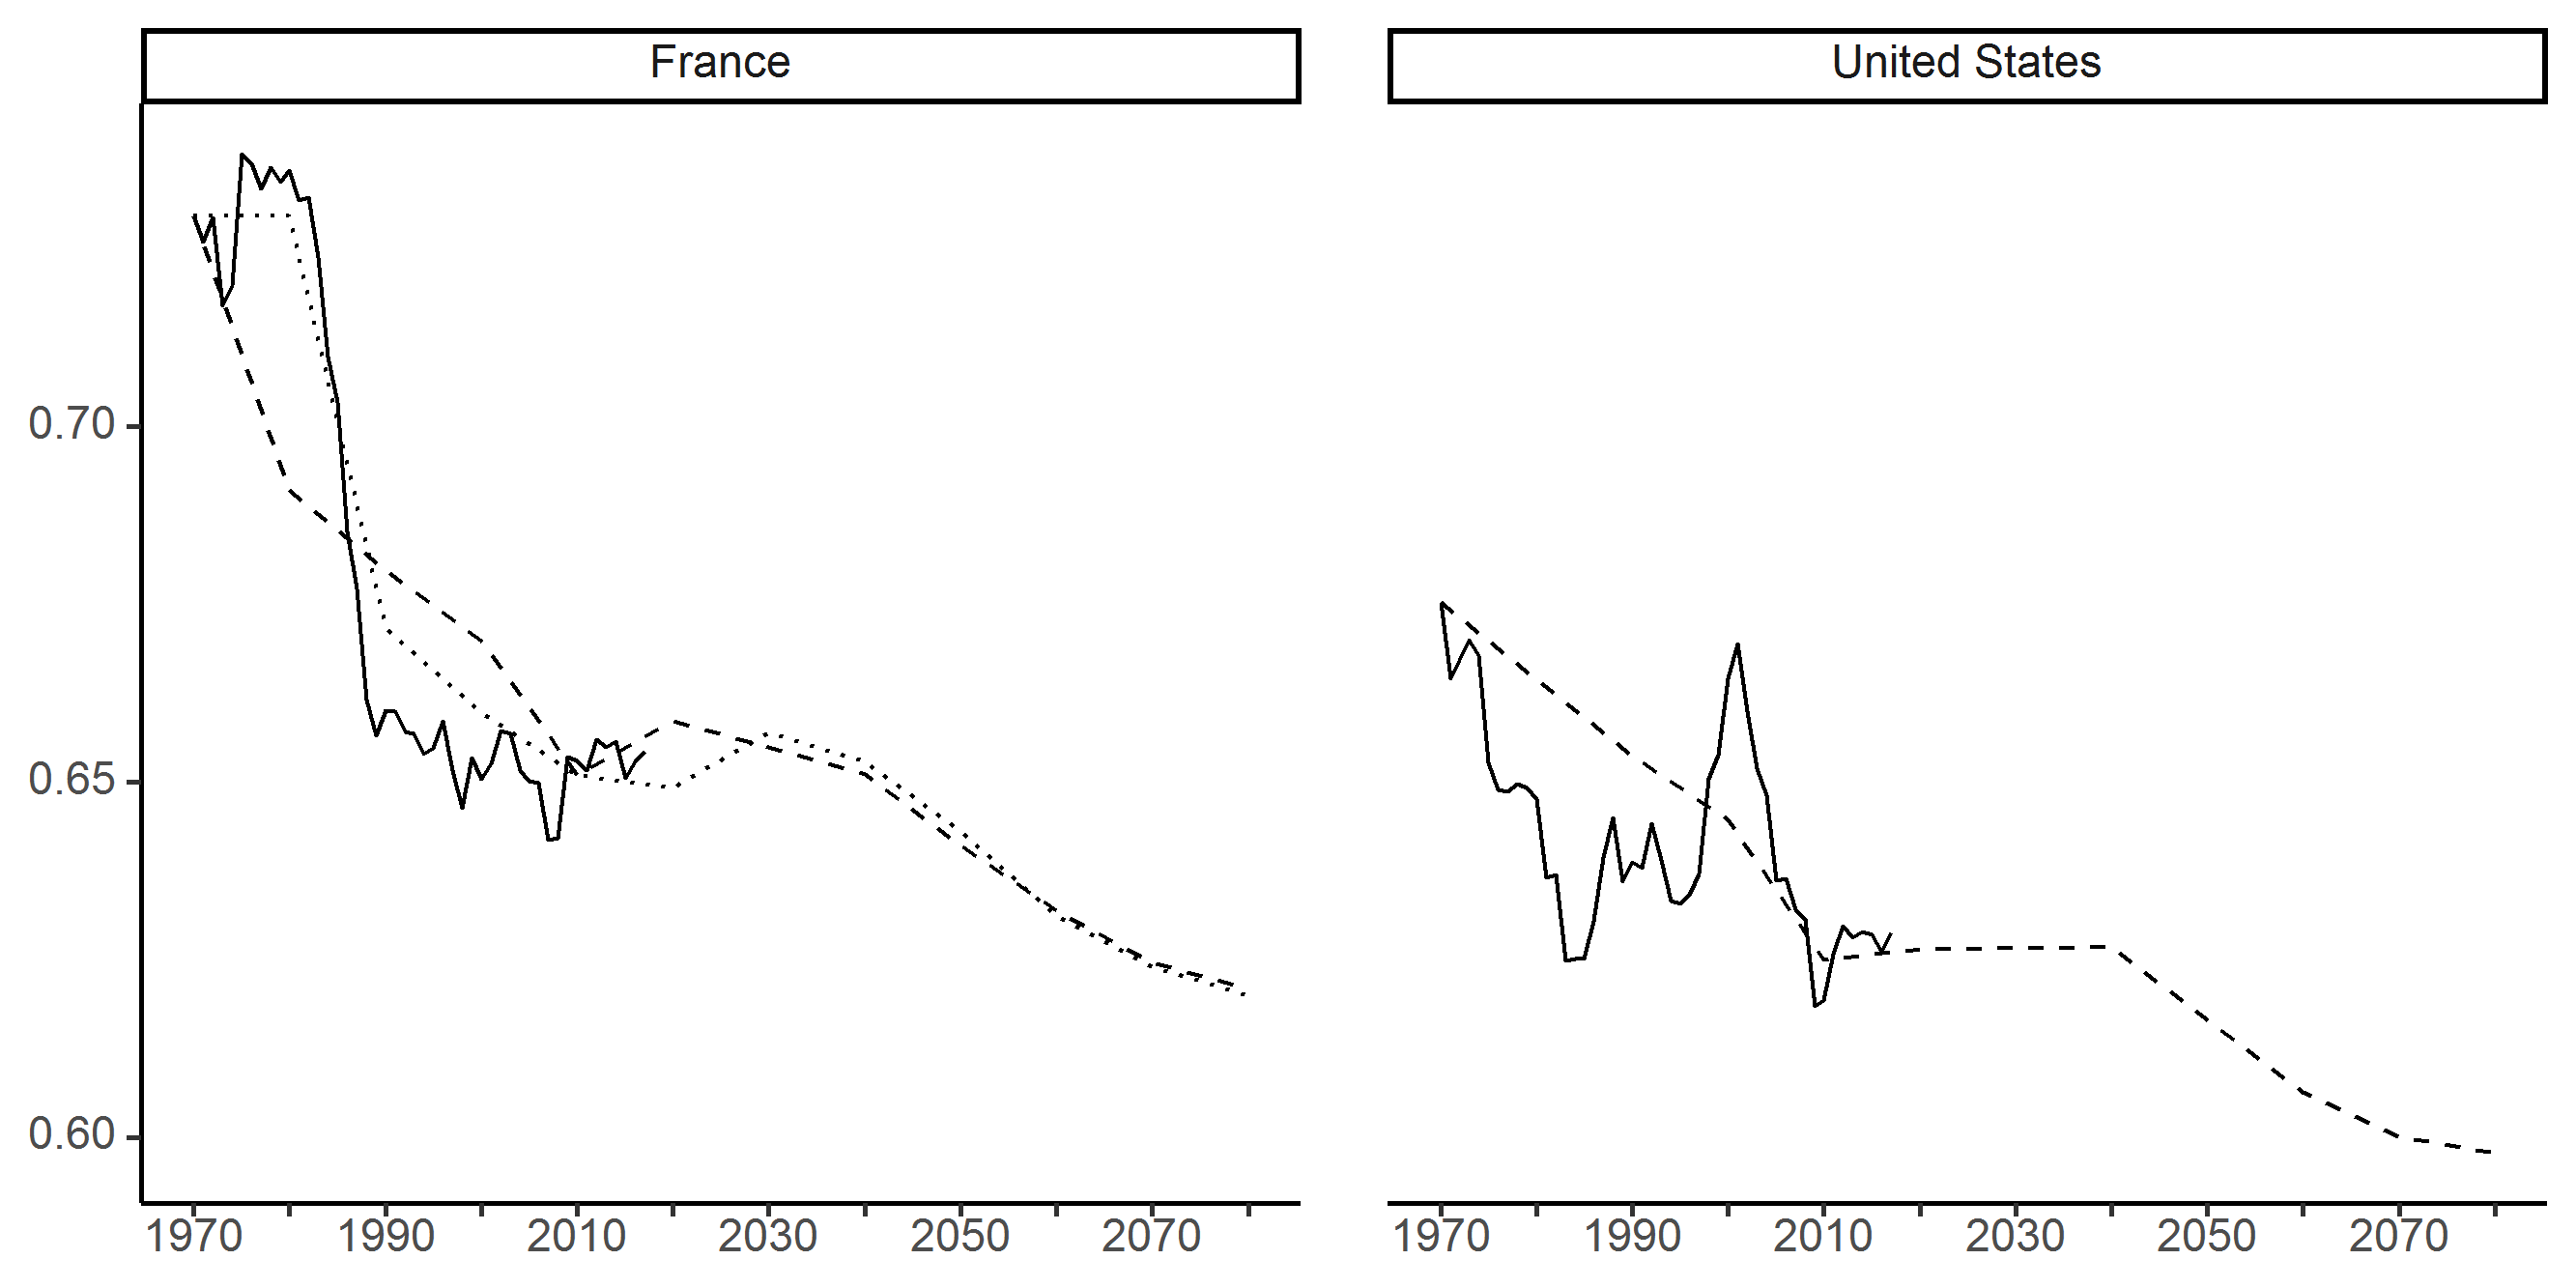
\includegraphics[width=1\linewidth]{../result/baseline7080.png}
	\caption{Model prediction of the labor share}
	\label{fig:baseline1080}
	\vspace{.5ex}
	\hrule
	\vspace{-4ex}
	\justify\singlespacing\footnotesize \textit{Notes:} The reader is referred to the footnote of the figure \ref{fig:baseline7010} for the legend of the curves.
\end{figure}
The model predicts that the labor share should continue to decline during the next decades in both countries. However, France should face a slight rise in 2020 up to 65.9 \% before to shrink again.\footnote{Under the model specification with a break in the regime of $\sigma$ for France (i.e. the dotted curve), the peak occurs in 2030 with a labor share up to 66.1 \%.} While the US labor share should remain stable around 62.6 \% between 2010 and 2040 and then follow the same pattern.

\subsubsection{Mechanisms of the resurgence}

The demographic context over the period 2010-2080, as presented in figure \ref{fig:demo}, is roughly the same for France and the United-States. The population growth $n_t$ faces a sharp decline between 2010 and 2050 before to stabilize thereafter. Meanwhile, the survival rate $p_t$ grows around 4\% per decades on average. Thus, the old-age-dependency ratio skyrockets until 2050. Once the population growth becomes stable, the ratio still grows but at a lower rate. This important aging of the population is mainly due to the baby-boomers' retirement. As a result of this demographic context, the youth political weight $\eta_t$ never gets back to its 2010's level and will strongly decline until 2050 for both countries.

% The story is the opposite of the period 1970-2010.

% Public Policy
Figure \ref{fig:dev_public1080} displays the deviation from the 1970 steady-state of public policy variables in percentage.
\begin{figure}[tb]
	\centering
	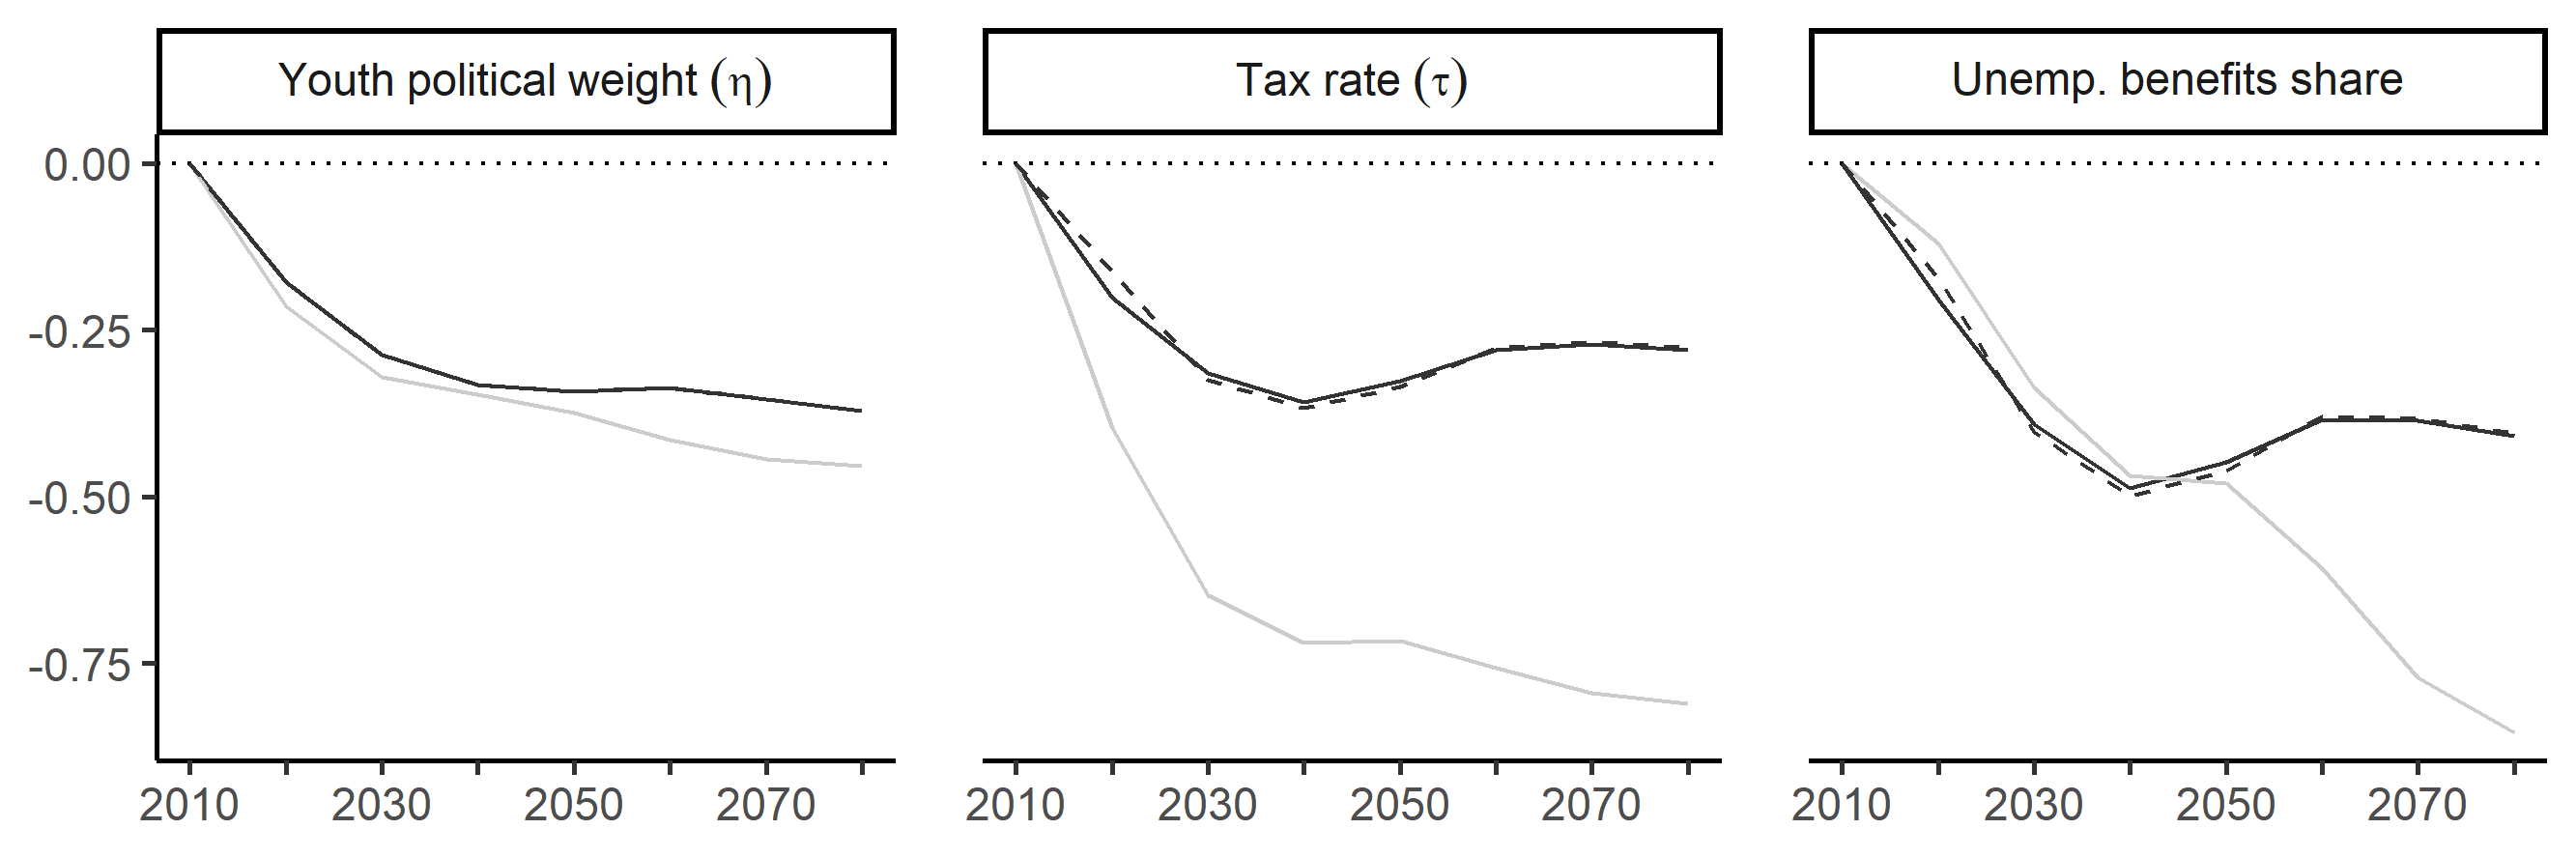
\includegraphics[width=1\linewidth]{../result/deviation/dev_public1080.png}
	\caption{Deviation from the 2010 steady-state of public policy variables}
	\label{fig:dev_public1080}
	\vspace{.5ex}
	\hrule
	\vspace{-4ex}
	\justify\singlespacing\footnotesize \textit{Notes:} The unemp. benefits share corresponds to the share of the unemployment benefits in the government spending, i.e. $buN^y/(\tau Y)$. The reader is referred to the footnote of the figure \ref{fig:dev_public7010} for the legend of the curves.
\end{figure}
The young political weight $\eta_t$ sharply declines due to the aging of the population. Thus, opportunist political candidates favor old households who desire less redistribution (i.e. $\partial\tau_t / \partial \eta_t > 0)$. Pro-elderly public policies are implemented. In terms of the model, it is translated by an increase of the health spending share in government revenue at the cost of the unemployment benefits one $b~share$.

% Wage bargaining
These policy changes interact with the wage bargaining because they affect the outside option of young households. Figure \ref{fig:dev_bargain1080} displays the deviation from the 2010 steady-state of wage bargaining variables in percentage.
\begin{figure}[!b]
	\centering
	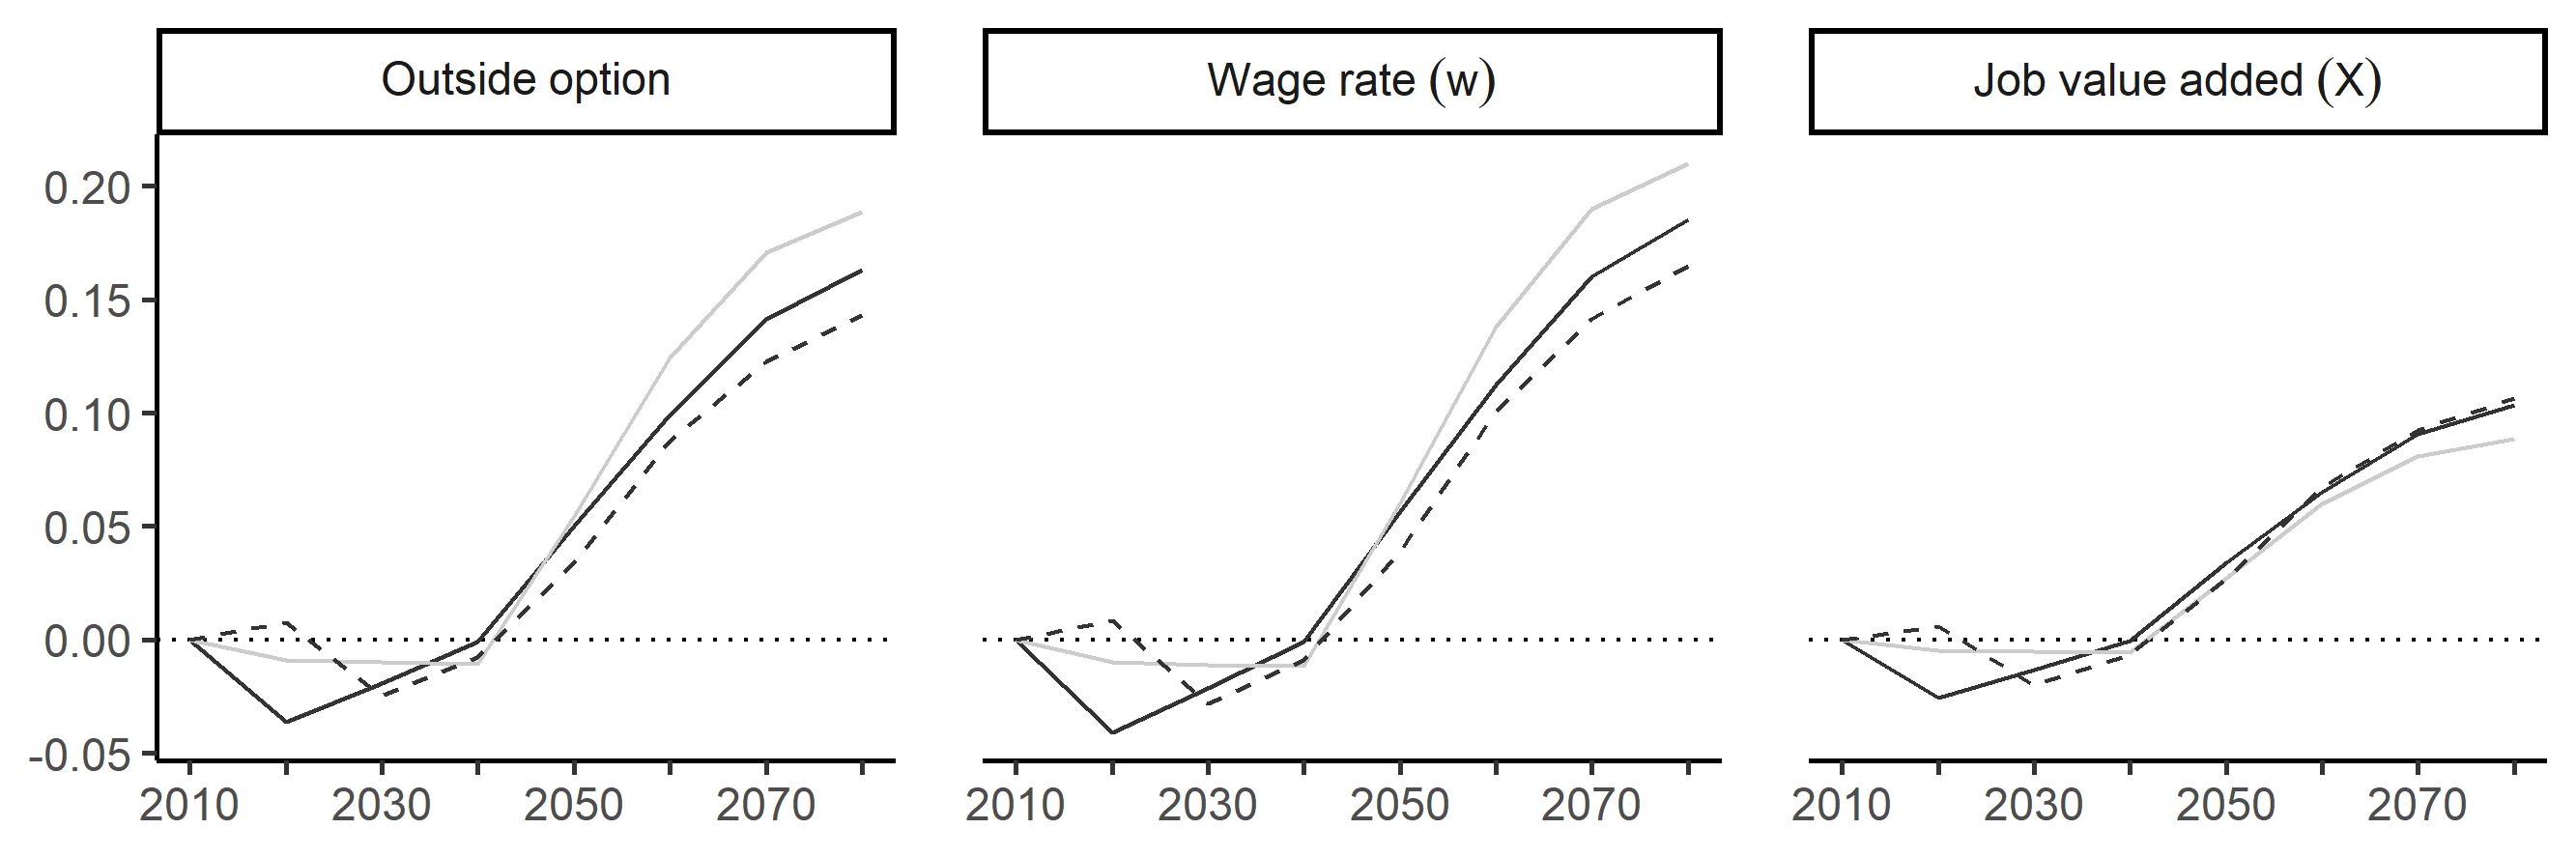
\includegraphics[width=1\linewidth]{../result/deviation/dev_bargain1080.png}
	\caption{Deviation from the 2010 steady-state of wage bargaining variables}
	\label{fig:dev_bargain1080}
	\vspace{.5ex}
	\hrule
	\vspace{-4ex}
	\justify\singlespacing\footnotesize \textit{Notes:} The outside option corresponds to $b/(1-\tau)$. The reader is referred to the footnote of the figure \ref{fig:dev_public7010} for the legend of the curves.
\end{figure}
Pro-elderly public policies leads to slightly weaken the outside option $b_t/(1-\tau_t)$ within the wage bargaining for both countries between 2010 and 2050. Workers are no longer in position to bargain greater wages and have to concede a wage cut. Hence, having a job between 2010 and 2050 is less worth in terms of utility as it was worth in 2010. But the drawback is not that tough because the declining wage goes along with a decline of the tax rate. In both countries, the outside option rises over the period 2050-2080 and so does the bargained wage. This increase is mainly due to the disappearance of baby-boomers. Thus, the age-related conflict within the public policy becomes relatively more in favor of the youth again.

% Production
Figure \ref{fig:dev_prod1080} displays the deviation from the 2010 steady-state of production function variables in percentage.
\begin{figure}[tb]
	\centering
	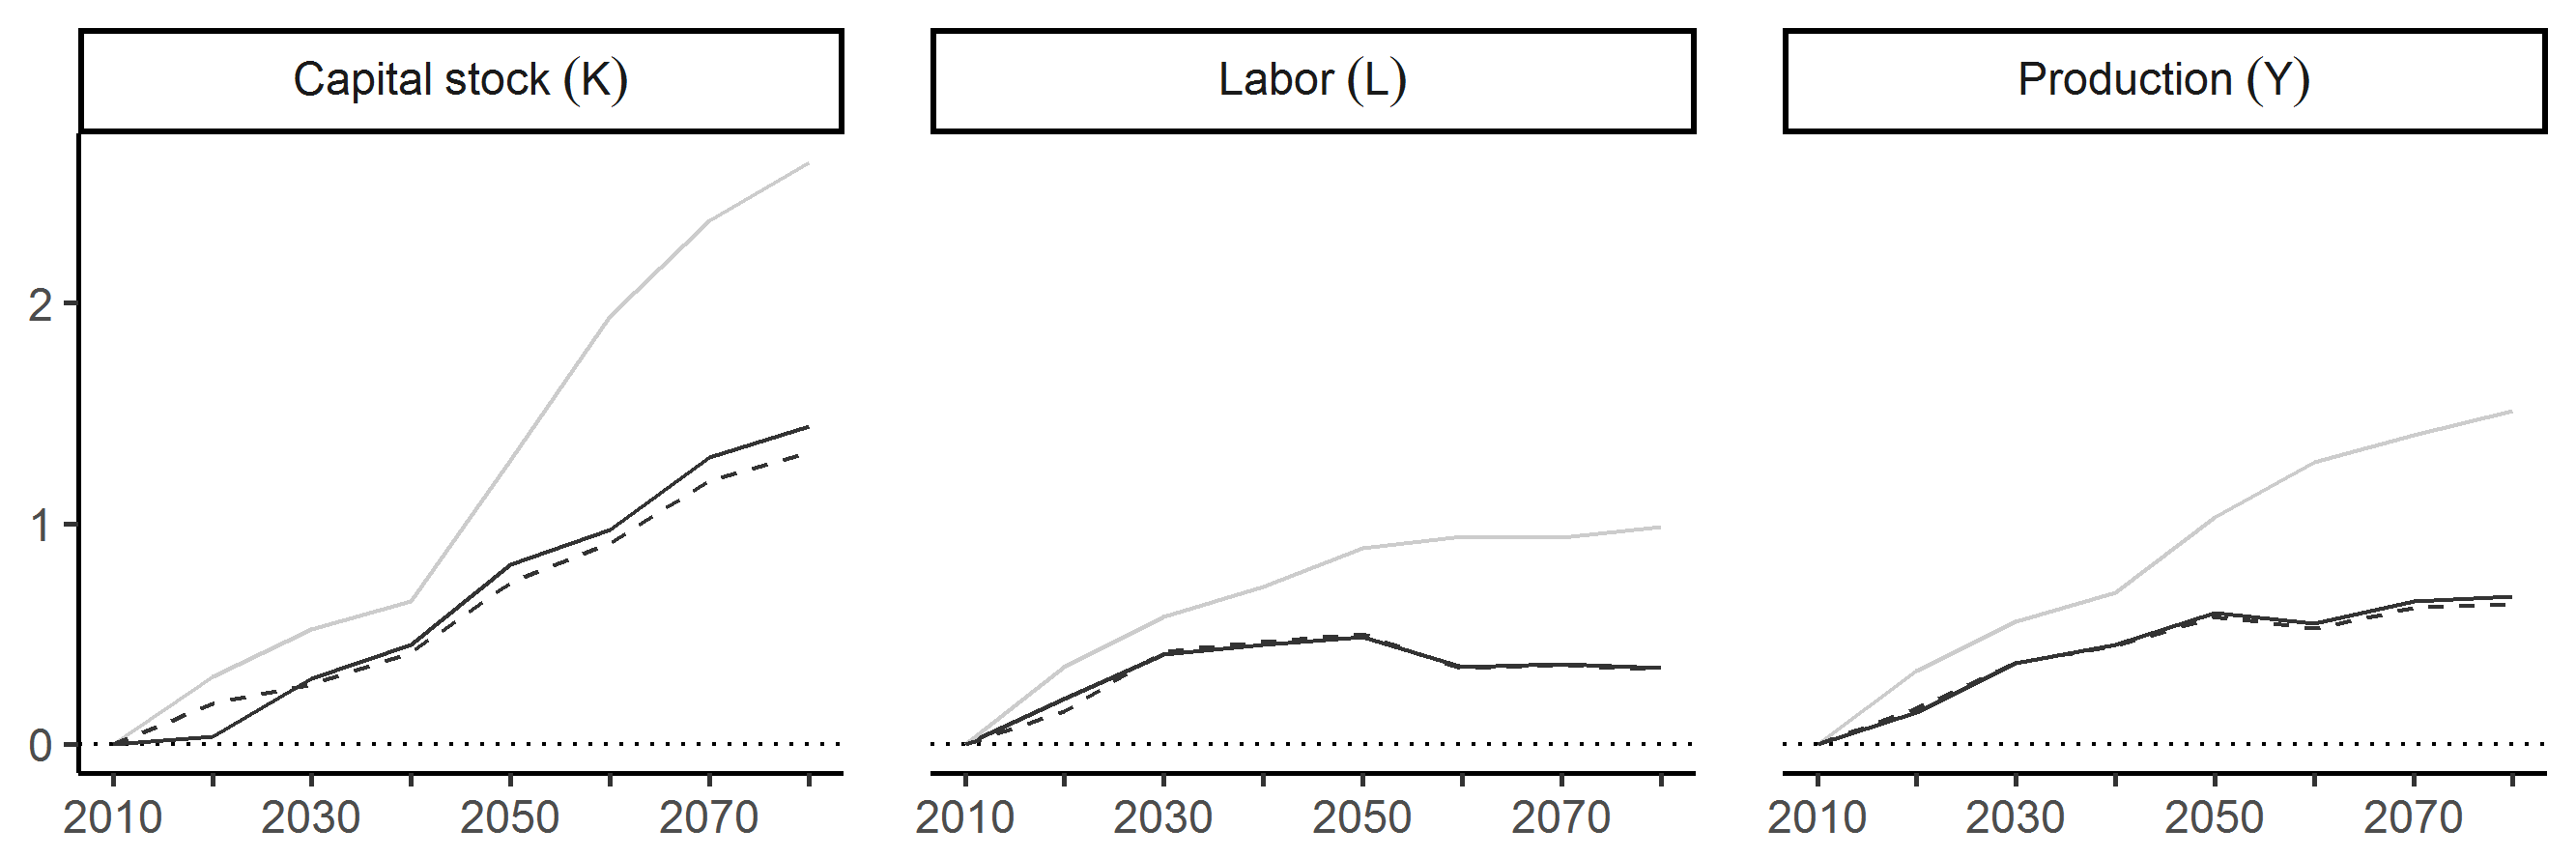
\includegraphics[width=1\linewidth]{../result/deviation/dev_prod1080.png}
	\caption{Deviation from the 1970 steady-state of production function variables}
	\label{fig:dev_prod1080}
	\vspace{.5ex}
	\hrule
	\vspace{-4ex}
	\justify\singlespacing\footnotesize \textit{Notes:} The reader is referred to the footnote of the figure \ref{fig:dev_public7010} for the legend of the curves.
\end{figure}
As the wage decreases between 2010 and 2050, the representative firm has incentive to hire. Thus, the labor $L_t$ does increase over this period. Meanwhile, the capital stock $K_t$ has increased due to savings $S_t$ of the previous periods. Thus, both input factors increase and so does the production $Y_t$. After 2050, France and the United-States diverge in their trajectories. On one hand, the US capital stock rises due to high savings of the previous periods.\footnote{This increase in savings owes to the baby-boomers cohort when they were young. Their massive entry on the labor market, rising expected life expectancy and higher wages have fostered savings and therefore the capital available in the economy once old.} This rise is strong enough to foster the representative firm to hire workers. Thus, the substitution mechanism does not undertake. On the other hand, the increase of the French capital stock does not follow the same exploding pattern. The french representative firm, as during the end of the twentieth century, shifts away from labor and decreases the number of workers. This divergence also appears on the labor market.

% Unemployment
Figure \ref{fig:dev_unemp1080} displays the deviation from the 2010 steady-state of unemployment's component variables in percentage.
\begin{figure}[tb]
	\centering
	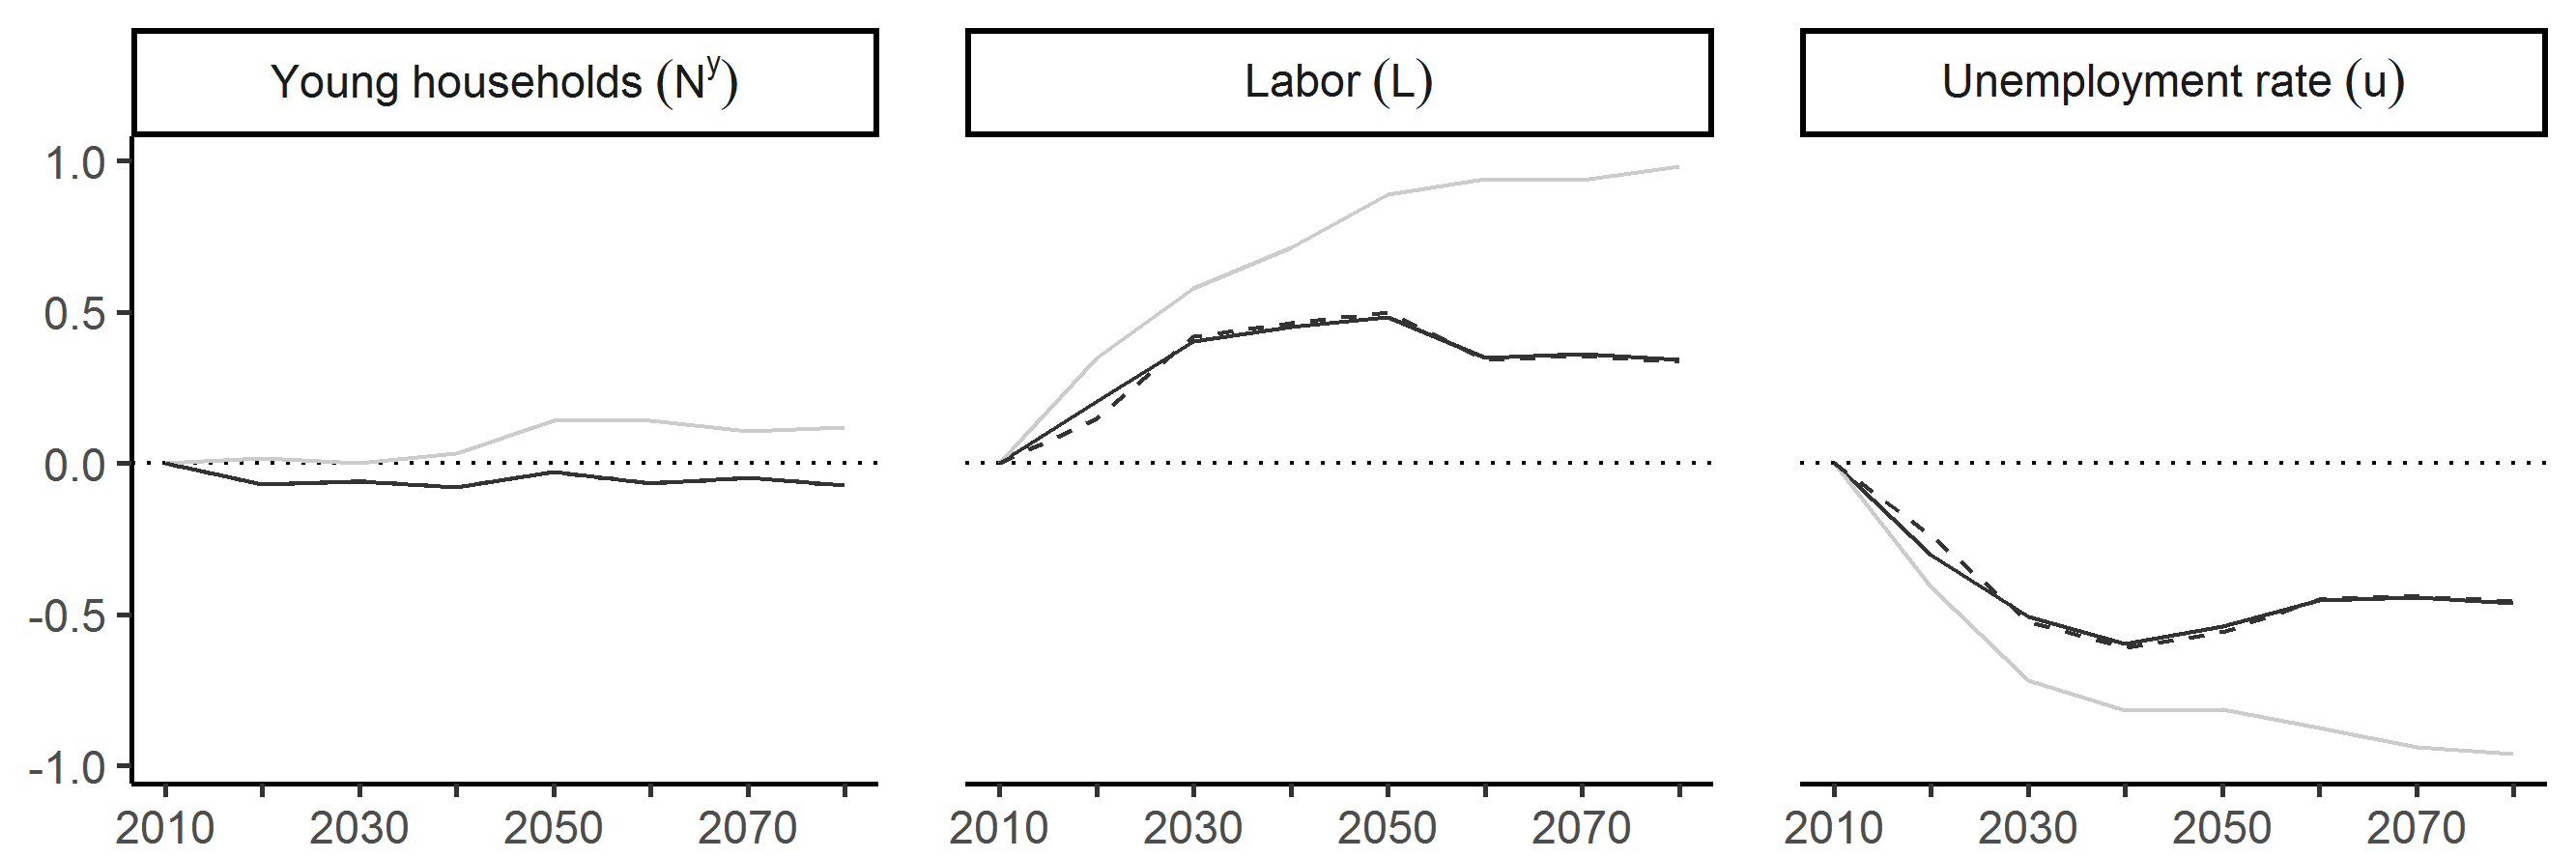
\includegraphics[width=1\linewidth]{../result/deviation/dev_unemp1080.png}
	\caption{Deviation from the 2010 steady-state of unemployment's component variables}
	\label{fig:dev_unemp1080}
	\vspace{.5ex}
	\hrule
	\vspace{-4ex}
	\justify\singlespacing\footnotesize \textit{Notes:} The reader is referred to the footnote of the figure \ref{fig:dev_public7010} for the legend of the curves.
\end{figure}
The labor force $N^y_t$ is roughly constant over the whole period and France is even below its 2010's level. Thus, the number of workers variations $L_t$ mainly drives the unemployment ones. The unemployment rate decreases in the United-States over the whole period. It falls down to 1.69\% by 2080 against 44.6\% in 2010. Here again, the sharp increase of the capital stock fosters employment until almost full-employment. The french unemployment rate decreases until 2050 before to slightly rise a bit and stabilize itself around 26.9\% in 2080.

% Labor share
Figure \ref{fig:dev_laborshare1080} displays the deviation from the 2010 steady-state of labor share's component variables in percentage.
\begin{figure}[tb]
	\centering
	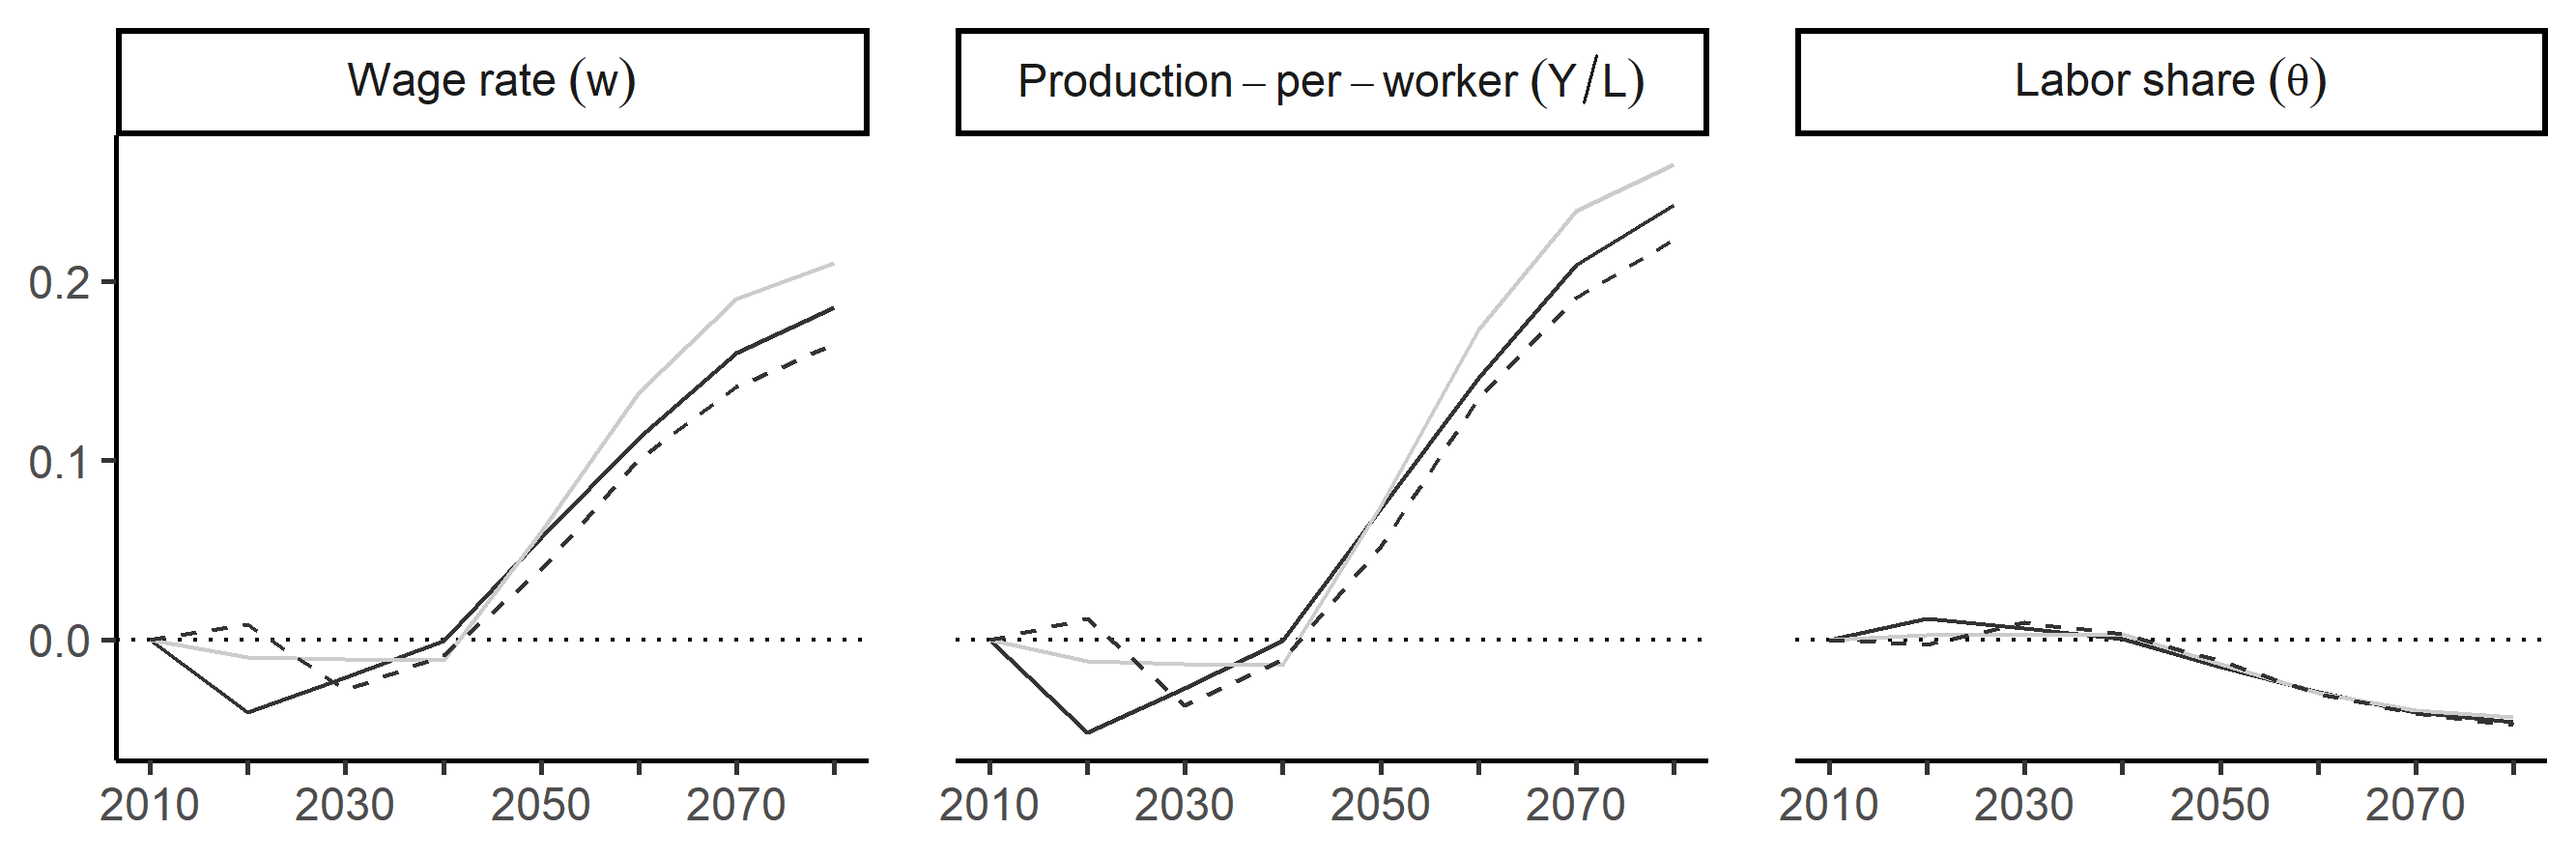
\includegraphics[width=1\linewidth]{../result/deviation/dev_laborshare1080.png}
	\caption{Deviation from the 2010 steady-state of labor share's component variables}
	\label{fig:dev_laborshare1080}
	\vspace{.5ex}
	\hrule
	\vspace{-4ex}
	\justify\singlespacing\footnotesize \textit{Notes:} The reader is referred to the footnote of the figure \ref{fig:dev_public7010} for the legend of the curves.
\end{figure}
French and US workers experience a minor reduction of their wage $w_t$ between 2010 and 2050 and so does the output-per-worker $Y_t/L_t$. The latter being greater than the former, the French labor share slightly increases. The US labor share remains constant because both variations compensate. After 2050, both labor shares decline to reach 62\% and 59.8\%, respectively for France and the United-States. While their respective levels in 2010 were 65.1\% and 62.5\%.

\subsection{Counterfactual and aging effect decomposition} \label{subsec:counterfactual}

So far, I have highlighted the different mechanisms through which the age structure of the population affects economic variables and therefore the labor share. For the remaining part of the paper, I consider that the previous model prediction is the benchmark prediction. For the french case, I envisage the model specification with a break in the regime of $\sigma$. To summarize, demographic changes are due to two determinant variables in the model : the population growth $n_t$ and the survival rate $p_t$. These variations may affect the labor share through two channels : the direct cohort effect $n_t$, $p_t$, $p_{t+1}$ and the indirect cohort effect $\eta_t(n_t, p_t, p_{t+1})$.

I make counterfactual predictions in order to quantity the respective role of each determinants and channels. The principle is to neutralize either a determinant of the demographic change or a channel through which the labor share is affected. The intuition behind the counterfactual is to observe what would have happened in terms of model predictions if this effect/channel was neutralized. By comparing a counterfactual simulation to the benchmark one, I can quantify its extent. I proceed in two steps. First, I examine the impact of the different determinants of demographic changes (i.e. $n_t$ versus $p_t$). Second, I investigate through which channels it occurs (i.e. direct versus indirect).

\subsubsection{Survival rate and population growth effects}

To neutralize the impact of the survival rate $p_t$, I assume that it remains at its 1970's level. Thus, $p_t = p_{1970}$ and $p_{t+1} = p_{2010}$. Old household population size is recalculated such that ${N^o_t}^\prime = N_t^o\times\frac{p_{1970}}{p_t}$. Moreover, $\eta_t = \frac{n_t}{p_{1970}}\frac{1+\alpha p_{2010}}{\omega}$.
%\footnote{For the first sequence of the model: 1970, 2010, 2050, \dots . The expected survival rate $p_{t+1}$ in 1970 is not equal to $p_{1970}$ but to $p_{2010}$. This exception is done in order to match the benchmark simulation in 1970 and thus share the same fixed point. Otherwise, $\eta^{\text{bench.}}_{1970} \neq \eta^{p}_{1970} \Rightarrow k^{\text{bench.}}_{1970} \neq k^{p}_{1970} \Rightarrow \theta^{\text{bench.}}_{1970} \neq \theta^{p}_{1970}$, where $^\text{bench.}$ stands for the benchmark simulation and $^p$ for the constant survival rate simulation.}
The other demographic variables (i.e. $n_t$ and $N^y_t$) follow the time series of the benchmark simulation. The initial capital stocks of the four sequences are also recalculated such that $K_0^\prime = \frac{1+\alpha p_t}{p_t}\frac{p_{1970}}{1+\alpha p_{1970}} K_0$.\footnote{Setting constant the survival rate implies changes in the saving rate through the expected survival rate $p_{t+1}$. $K_0 \equiv S_{-1} = \frac{\alpha p_0}{1+\alpha p_0}\left[(1-\tau_{-1})w_{-1}(1-u_{-1})+b_{-1}u_{-1}\right]N_{-1}^y$. In order to assess the true impact of the survival rate, it is also necessary to consider saving rate changes in the counterfactual simulation. Thus, the initial capital stocks for the first periods of the four sequences becomes $K_0^\prime = \frac{1+\alpha p_t}{p_t}\frac{p_{1970}}{1+\alpha p_{1970}} K_0$. Notice that a change in the survival rate $p_0$ should also affect the aggregated disposable income of young households in $t=-1$, i.e. $(1-\tau_{-1})w_{-1}(1-u_{-1})+b_{-1}u_{-1}$. However, I do not consider this source of change. Notice also that the term $N_{-1}^y$ does not change because $N_{-1}^y = \frac{N_0^o}{p_0} = \frac{{N_0^o}^\prime}{p_{1970}}$.} The methodology is analogous to neutralize the impact of the population growth but with $n_t = n_{1970}$, ${N_t^y}^\prime = N_t^y\times\frac{n_{1970}}{n_t}$ and $\eta_t = \frac{n_{1970}}{p_t}\frac{1+\alpha p_{t+1}}{\omega}$.\footnote{In this specification, the initial capital stocks are not changed because $n_0$ does not affect $S_{-1}$.} Finally, a last counterfactual is made to neutralize both effects. So, $p_t = p_{1970}$, $p_{t+1} = p_{2010}$, $n_t = n_{1970}$ and $\eta_t = \eta_{1970}$. As before, population sizes and initial capital stock values are recalculated.
%\footnote{The same exception, as explained in the previous footnote, is done to ensure that the labor share in matched in 1970.}
Here, the old-age-dependency ratio remains constant. Table \ref{tab:demo1970} summarizes demographic variables in 1970.
\begin{table}[tb]
	\caption{Demographic variables in 1970}\label{tab:demo1970}
	\centering
	\begin{threeparttable}
		\begin{tabular}{c l D{.}{.}{-3} D{.}{.}{-3}}
			\multicolumn{2}{c}{\textbf{Variable}} & \multicolumn{1}{r}{\textbf{France}} & \multicolumn{1}{r}{\textbf{United-States}}            \\ \hline \hline
			$p_{1970}$           	& Survival rate in 1970         					  & 0.417 & 0.476		\\
			$n_{1970}$          	& Population growth in 1970                           & 1.134 & 1.597		\\
			$p_{2010}$           	& Expected survival rate in 2010         			  & 0.583 & 0.561		\\
			$\frac{p_{1970}}{n_{1970}}$     & Old-age-dependency ratio in 1970         	  & 0.368 & 0.298			\\
			$\eta_{1970}$           & Youth political weight in 1970                      & 3.846 & 3.008		\\ \hline
			\hline
		\end{tabular}
	%	\vspace{-3ex}
	%	\begin{tablenotes}
	%		\vspace{-3ex}
	%		\singlespacing
	%		{\footnotesize
	%			\item \textit{Note :} .
	%		}
	%	\end{tablenotes}
	\end{threeparttable}
\end{table}

Figure \ref{fig:counter_PGSR_1970} displays the model predictions of the labor share with counterfactual specifications.
\begin{figure}[tb]
	\centering
	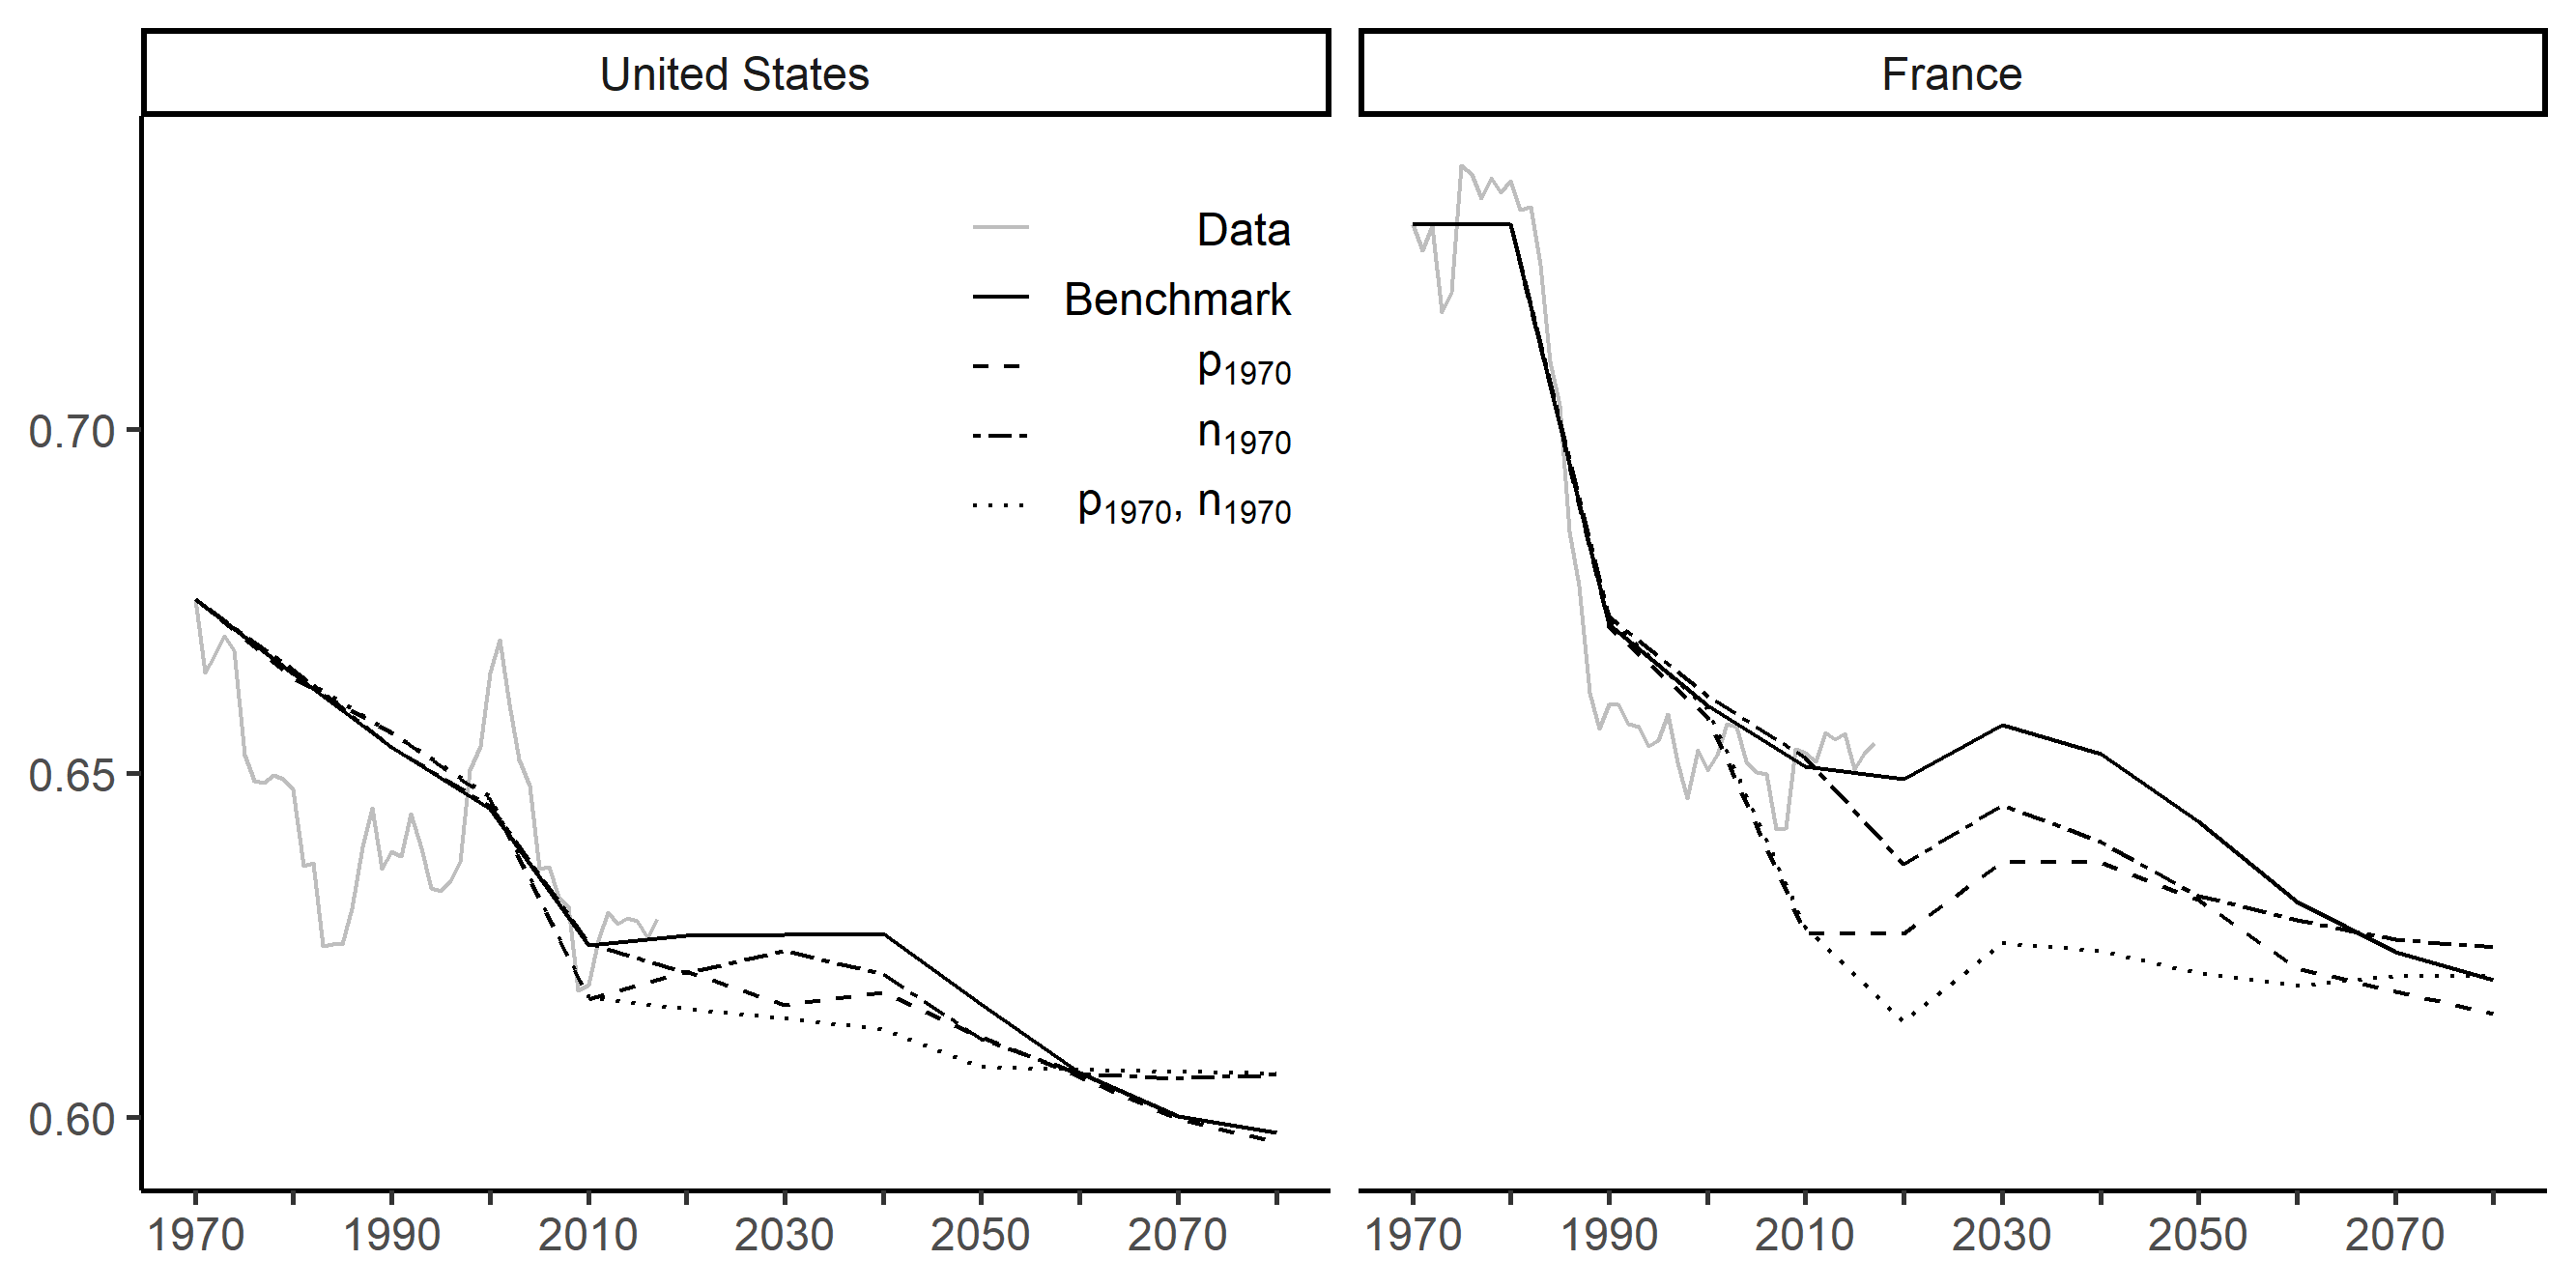
\includegraphics[width=1\linewidth]{../result/decomposition/counter_PGSR.png}
	\caption{Model predictions of the labor share with counterfactual specifications}
	\label{fig:counter_PGSR_1970}
%	\vspace{.5ex}
%	\hrule
%	\vspace{-4ex}
%	\justify\singlespacing\footnotesize 
\end{figure}
To interpret the role played by each demographic variable, I compare each counterfactual time series to the benchmark one. For instance, let start with the impact of the survival rate in France. I look at the dashed curve with respect to the solid one. This curve corresponds to the counterfactual where the survival rate $p_t$ and $p_{t+1}$ remain at their 1970's levels. So, if the survival rate would have not changed, then the labor share would have followed the dashed curve pattern. 
%The blue curve lies below the red one between 1980 and 2020 and above thereafter. Therefore, the survival rate dynamic had a positive impact on the labor share between 1980 and 2020 and a negative one thereafter.
The dashed curve lies below the solid one. Therefore, the survival rate dynamic has a positive impact on the labor share in both countries.
The way to interpret the other counterfactuals is similar.
The dash-dotted curve remains above the solid one until 2050 for France and 2030 for the United States. Until these years, the population growth dynamic has a negative impact on the labor share and a positive one thereafter.
Finally, the dotted curve which corresponds to the counterfactual where both effects are neutralized is below the benchmark simulation. Since 1970, all demographic dynamics have led to increase the labor share with respect to what it would have been without these dynamics.
However, this representation is tediously legible. Therefore, I compute the distance between the benchmark labor share and each counterfactual labor share. Using the Chasles' relation within an affine space at each point in time, it is possible to isolate the extent of each effect.\footnote{Let $r$ (resp. $b, g, p$) be the labor share from the red (resp. blue, green, purple) curve on figure \ref{fig:counter_PGSR_1970}. For a given year, $2\vec{rp} = \vec{rb} + \vec{bp} + \vec{rg} + \vec{gp} \Leftrightarrow \vec{rp} = \vec{rb} + \vec{rg} + \vec{\text{int.}}$, where $\vec{\text{int.}} \equiv \vec{bp} + \vec{gp} - \vec{rp} = \vec{gp} +\vec{br} = \vec{bp} + \vec{gr}$ is the interaction of both effects defined as the part which is not exclusively explained by both effects independently.} Figure \ref{fig:decomp_PGSR} displays the labors share's gap between the benchmark and the counterfactuals in percentage points.
\begin{figure}[tb]
	\centering
	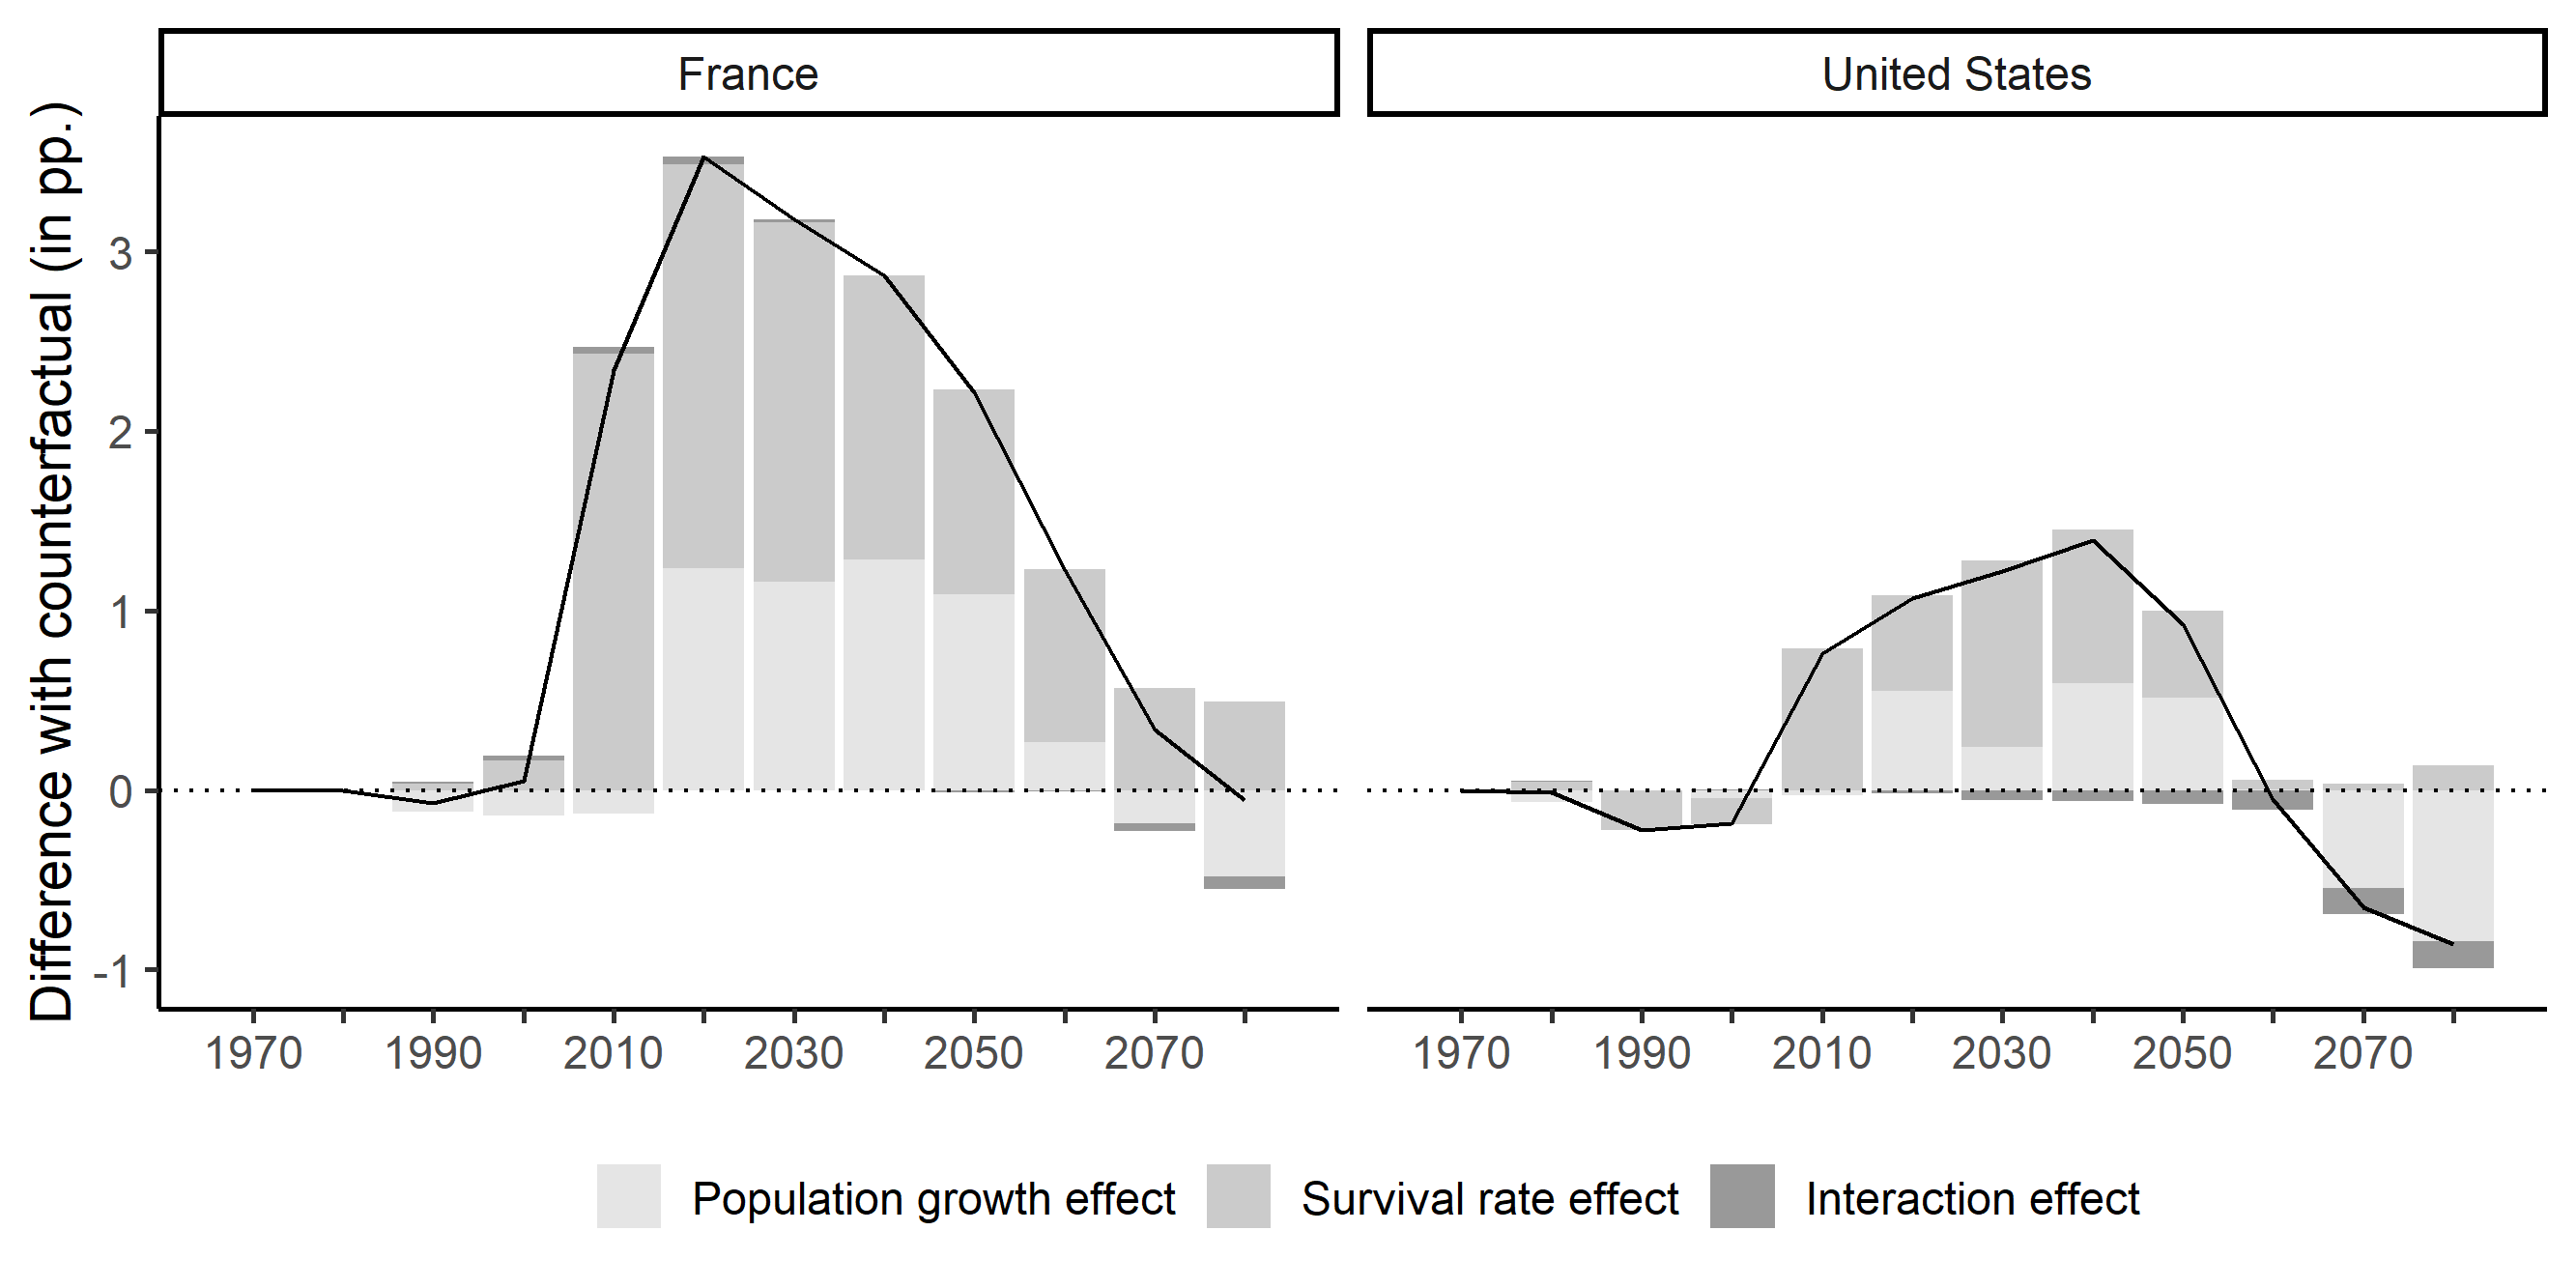
\includegraphics[width=1\linewidth]{../result/decomposition/decomp_PGSR.png}
	\caption{Aging-effect decomposition by determinants}
	\label{fig:decomp_PGSR}
	%	\vspace{.5ex}
	%	\hrule
	%	\vspace{-4ex}
	%	\justify\singlespacing\footnotesize 
\end{figure}
As mentioned above, the survival rate effect has kept the labor share relatively high in both countries. Another way to think about that is to consider demographic dynamics in terms of cohort sizes. Until 2010, if the survival rate had been held constant, then the massive increase in the population of young households due to the baby-boomers' presence would have generated an even larger decline of the labor share. However, the aging population (i.e. the increase of the survival rate) has thwarted part of this fall. Notice that the difference with the counterfactual is less than 1\% in the case of the United-States. It suggests that the aging phenomenon over this period is a larger determinant of the labor share in France compared to the United-States.
%After 2010, the explanation power of the survival rate falls and the distance between the benchmark simulation with respect to the counterfactual shrinks. It corresponds to the fact that demographic variations are not as wide as during the end of the 20th century.
The analysis of the determinants only reveals part of the explanation. It is also necessary to look at the channels that affect the labor share.

\subsubsection{Direct and indirect cohort effects}

To neutralize the indirect cohort effect, I fix the youth political weight $\eta_t$ to its 1970's value but I keep the demographic variables' time series $n_t$, $p_t$ and $p_{t+1}$ as in the benchmark simulation. Thus, $\eta_t = \eta_{1970}$. To neutralize the direct cohort effect, I assume that all the demographic variables remain at their 1970's level. Thus, $p_t = p_{1970}$, $p_{t+1} = p_{2010}$, $n_t = n_{1970}$ and population sizes but also initial capital stocks are recalculated. But the youth political weight time series $\eta_t$ is the one of the benchmark simulation. Finally, a last counterfactual is made where I neutralize both effects.\footnote{This last specification is the same as in the survival rate and population growth effects decomposition. So the purple curve in figure \ref{fig:counter_PGSR_1970}.}

Figure \ref{fig:counter_DEIE} displays the model predictions of the labor share with counterfactual specifications.
\begin{figure}[tb]
	\centering
	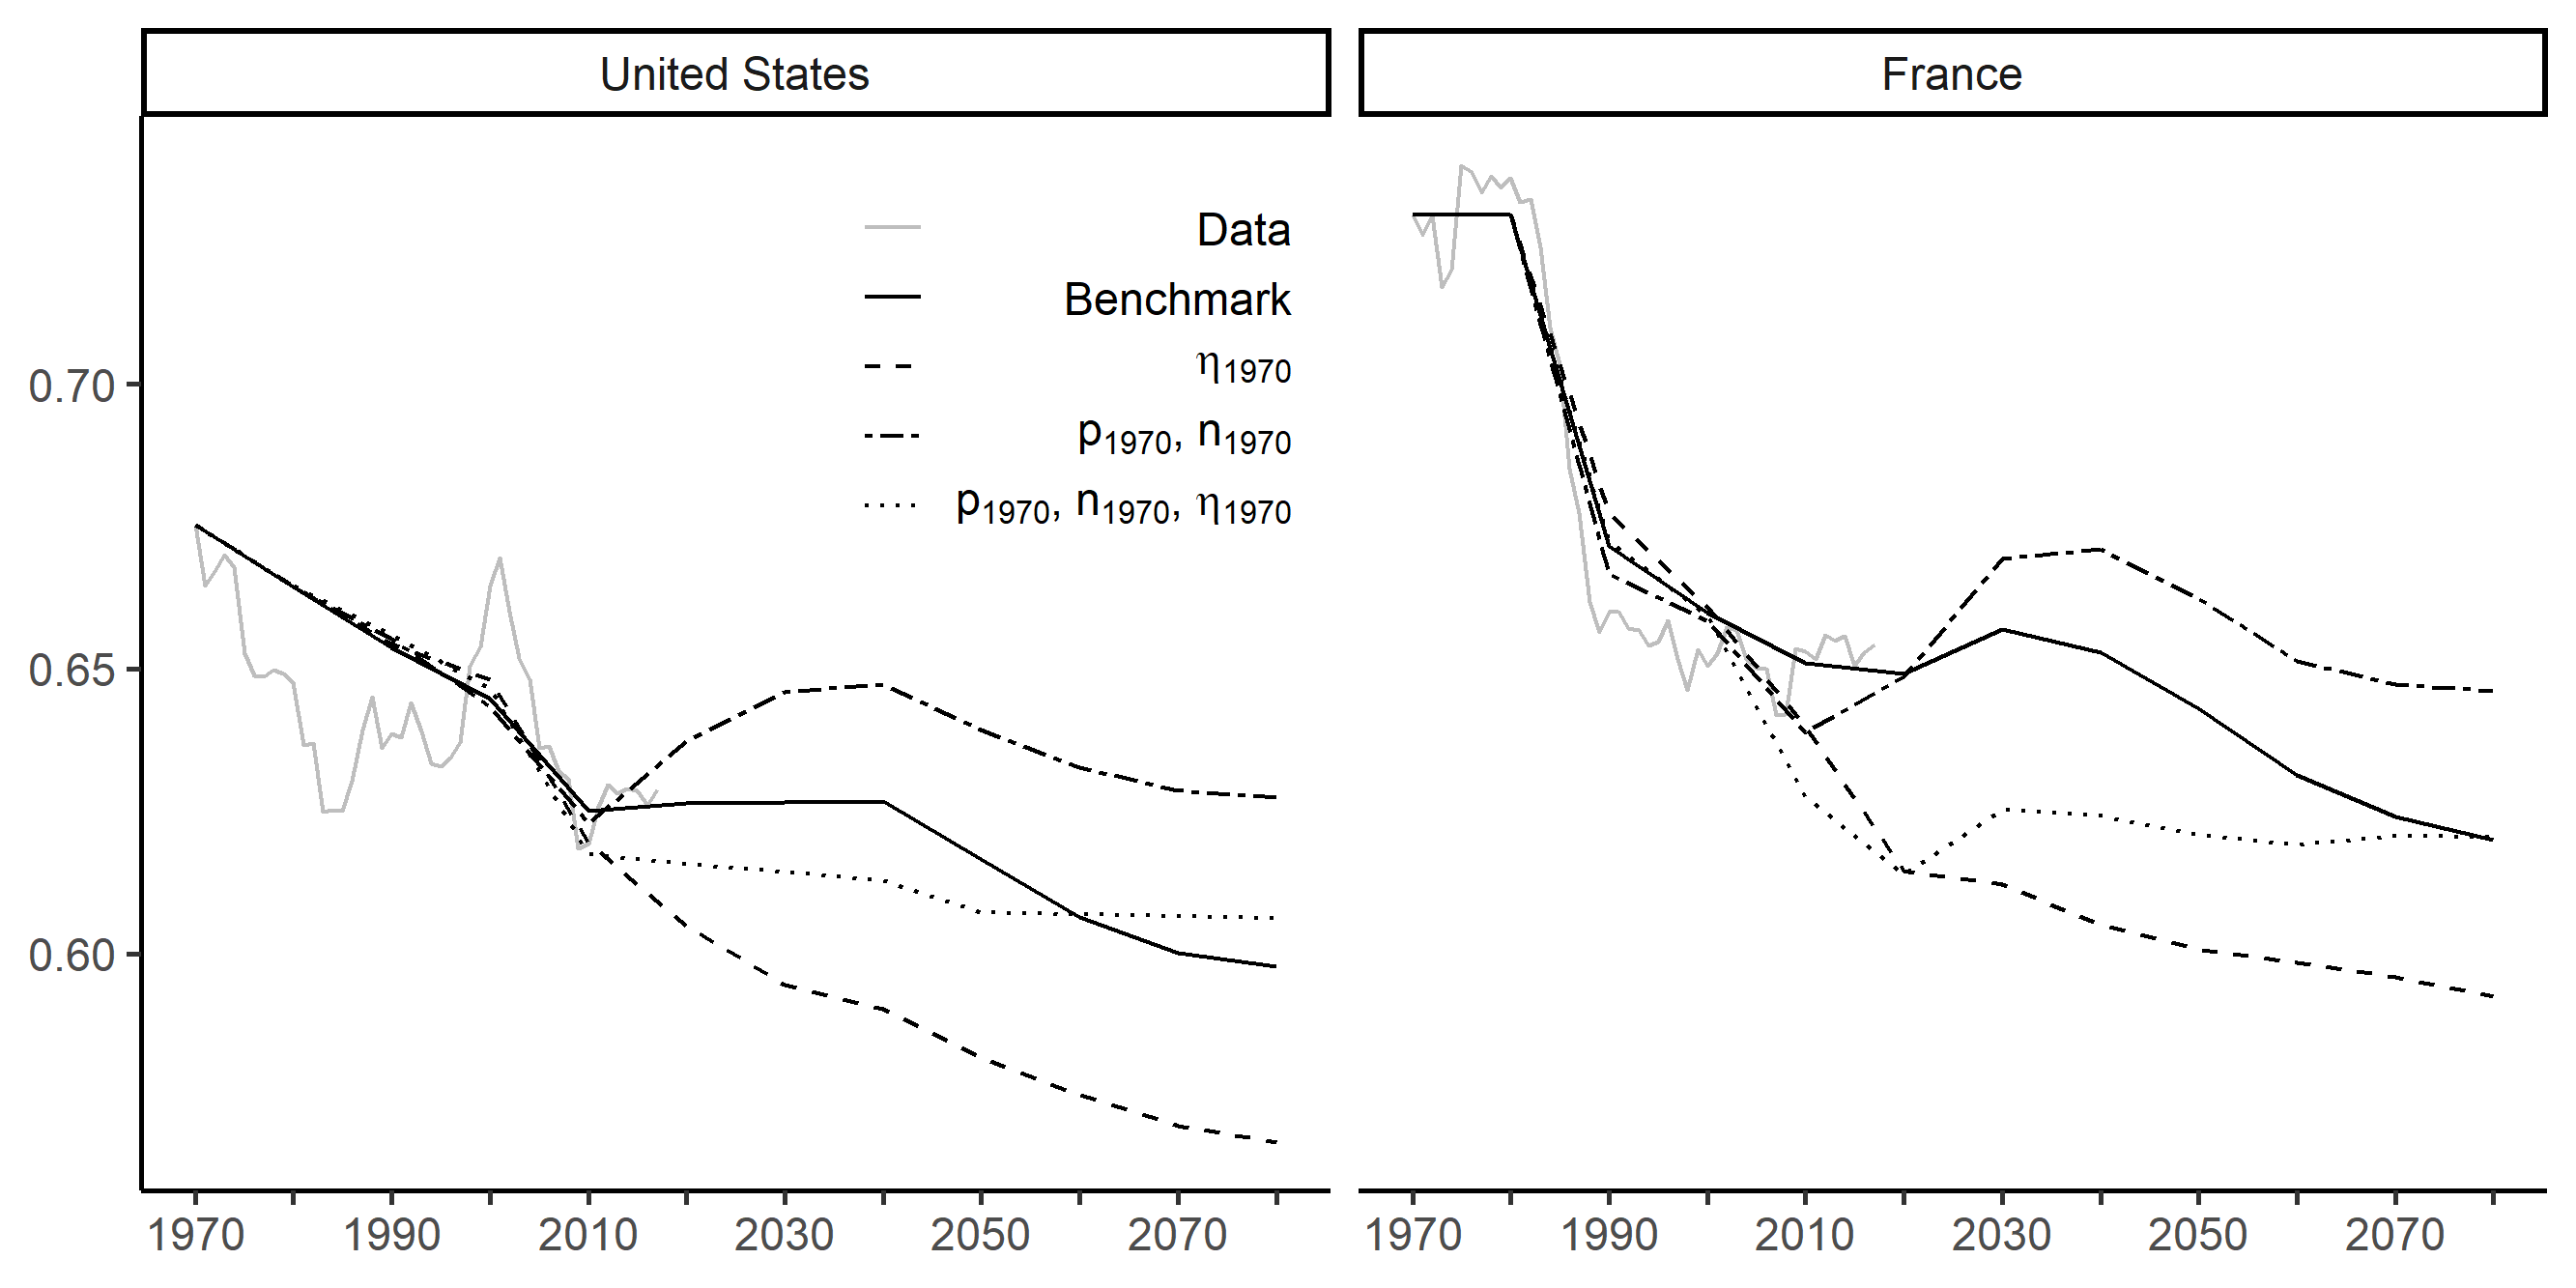
\includegraphics[width=1\linewidth]{../result/decomposition/counter_DEIE.png}
	\caption{Model predictions of the labor share with counterfactual specifications}
	\label{fig:counter_DEIE}
	%	\vspace{.5ex}
	%	\hrule
	%	\vspace{-4ex}
	%	\justify\singlespacing\footnotesize 
\end{figure}
The methodology to interpret this figure is similar to the one of the figure \ref{fig:counter_PGSR}. The dash-dotted curve corresponds to the direct cohort effect. For both countries, this curve is below the benchmark curve until 2010 and above thereafter. It means that the demographic dynamics' net impact through the direct channel is positive on the labor share until 2010 and negative thereafter. Looking at the dashed curve, it is slightly above before 2000 and largely below thereafter. The net impact of the indirect cohort effect is negative up to 2000 and positive subsequently. However, this representation is also tediously legible. Therefore, I isolate the extent of each channel with the same methodology as before. Figure \ref{fig:decomp_DEIE} displays the labor share's gap between the benchmark and the counterfactuals in percentage points.
\begin{figure}[tb]
	\centering
	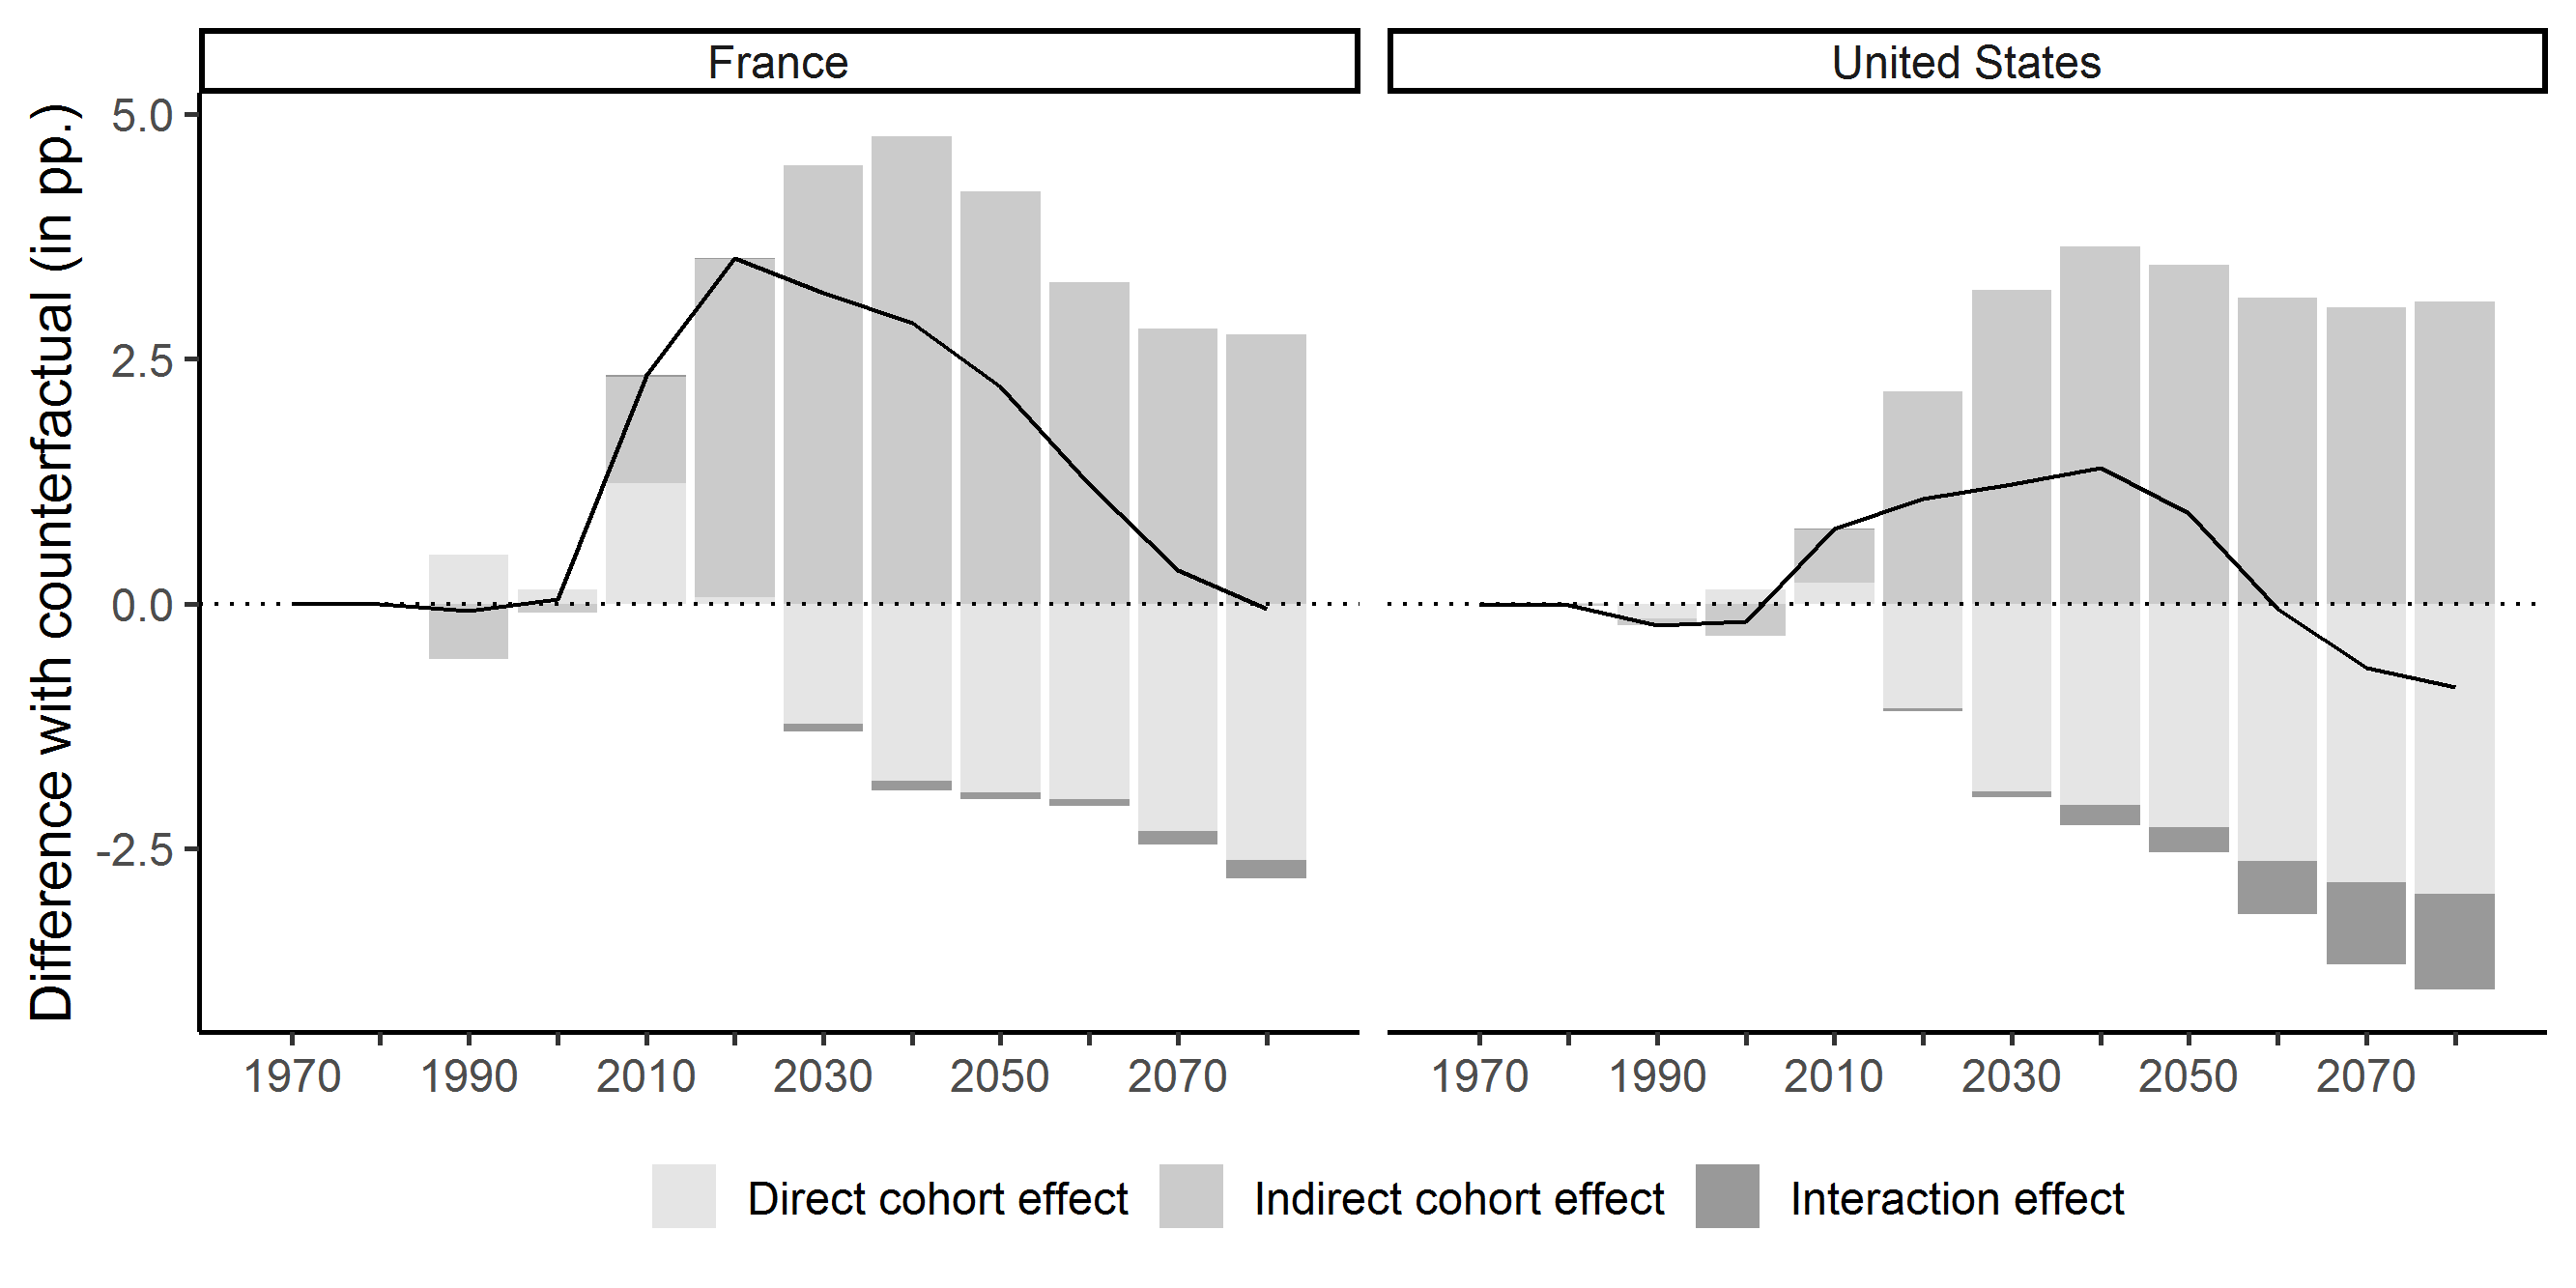
\includegraphics[width=1\linewidth]{../result/decomposition/decomp_DEIE.png}
	\caption{Aging-effect decomposition by channels}
	\label{fig:decomp_DEIE}
	%	\vspace{.5ex}
	%	\hrule
	%	\vspace{-4ex}
	%	\justify\singlespacing\footnotesize 
\end{figure}
The direct cohort effect is positive when the baby-boomers are young and after becomes negative. While the indirect cohort effect has the opposite pattern. The direct cohort effect dominates the indirect one until 2010 before to become less influential. Until 2010, if the demographic variables had been held constant, then the relatively high political power of the youth due to the baby-boomers' presence would have generated an even larger decline of the labor share. However, the aging population was mainly driven by the increasing survival rate which has thwarted part of the fall. Notice that, here again, the difference with counterfactual is less than 1\% in the case of the United-States. It suggests that the aging phenomenon over this period is a larger determinant of the labor share in France compared to the United-States.
% May be for the Summary
After 2010, so once the baby-boomers' cohort retires, the model predicts that the indirect cohort effect (i.e. the decline of the youth political power) should exceed the direct one. This is directly related to the mechanism analysis of section \ref{subsec:model_pred}. The baby-boomers and more generally the old households becomes the winners of the age-related conflict within the public policy over this period. Thereby, they reduce the workers' outside option which leads to a wage cut or more precisely to a wage stagnation. The labor cost remains constant while the capital available in the economy accumulates. It generates an incentive for the representative firm to hire more workers. As a result, the labor share increases.
% May be for the Summary

\subsubsection{Summary}

Figure \ref{fig:decomp_country_period} summarizes the aging-effect decomposition by periods and countries.
\begin{figure}[tb]
	\centering
	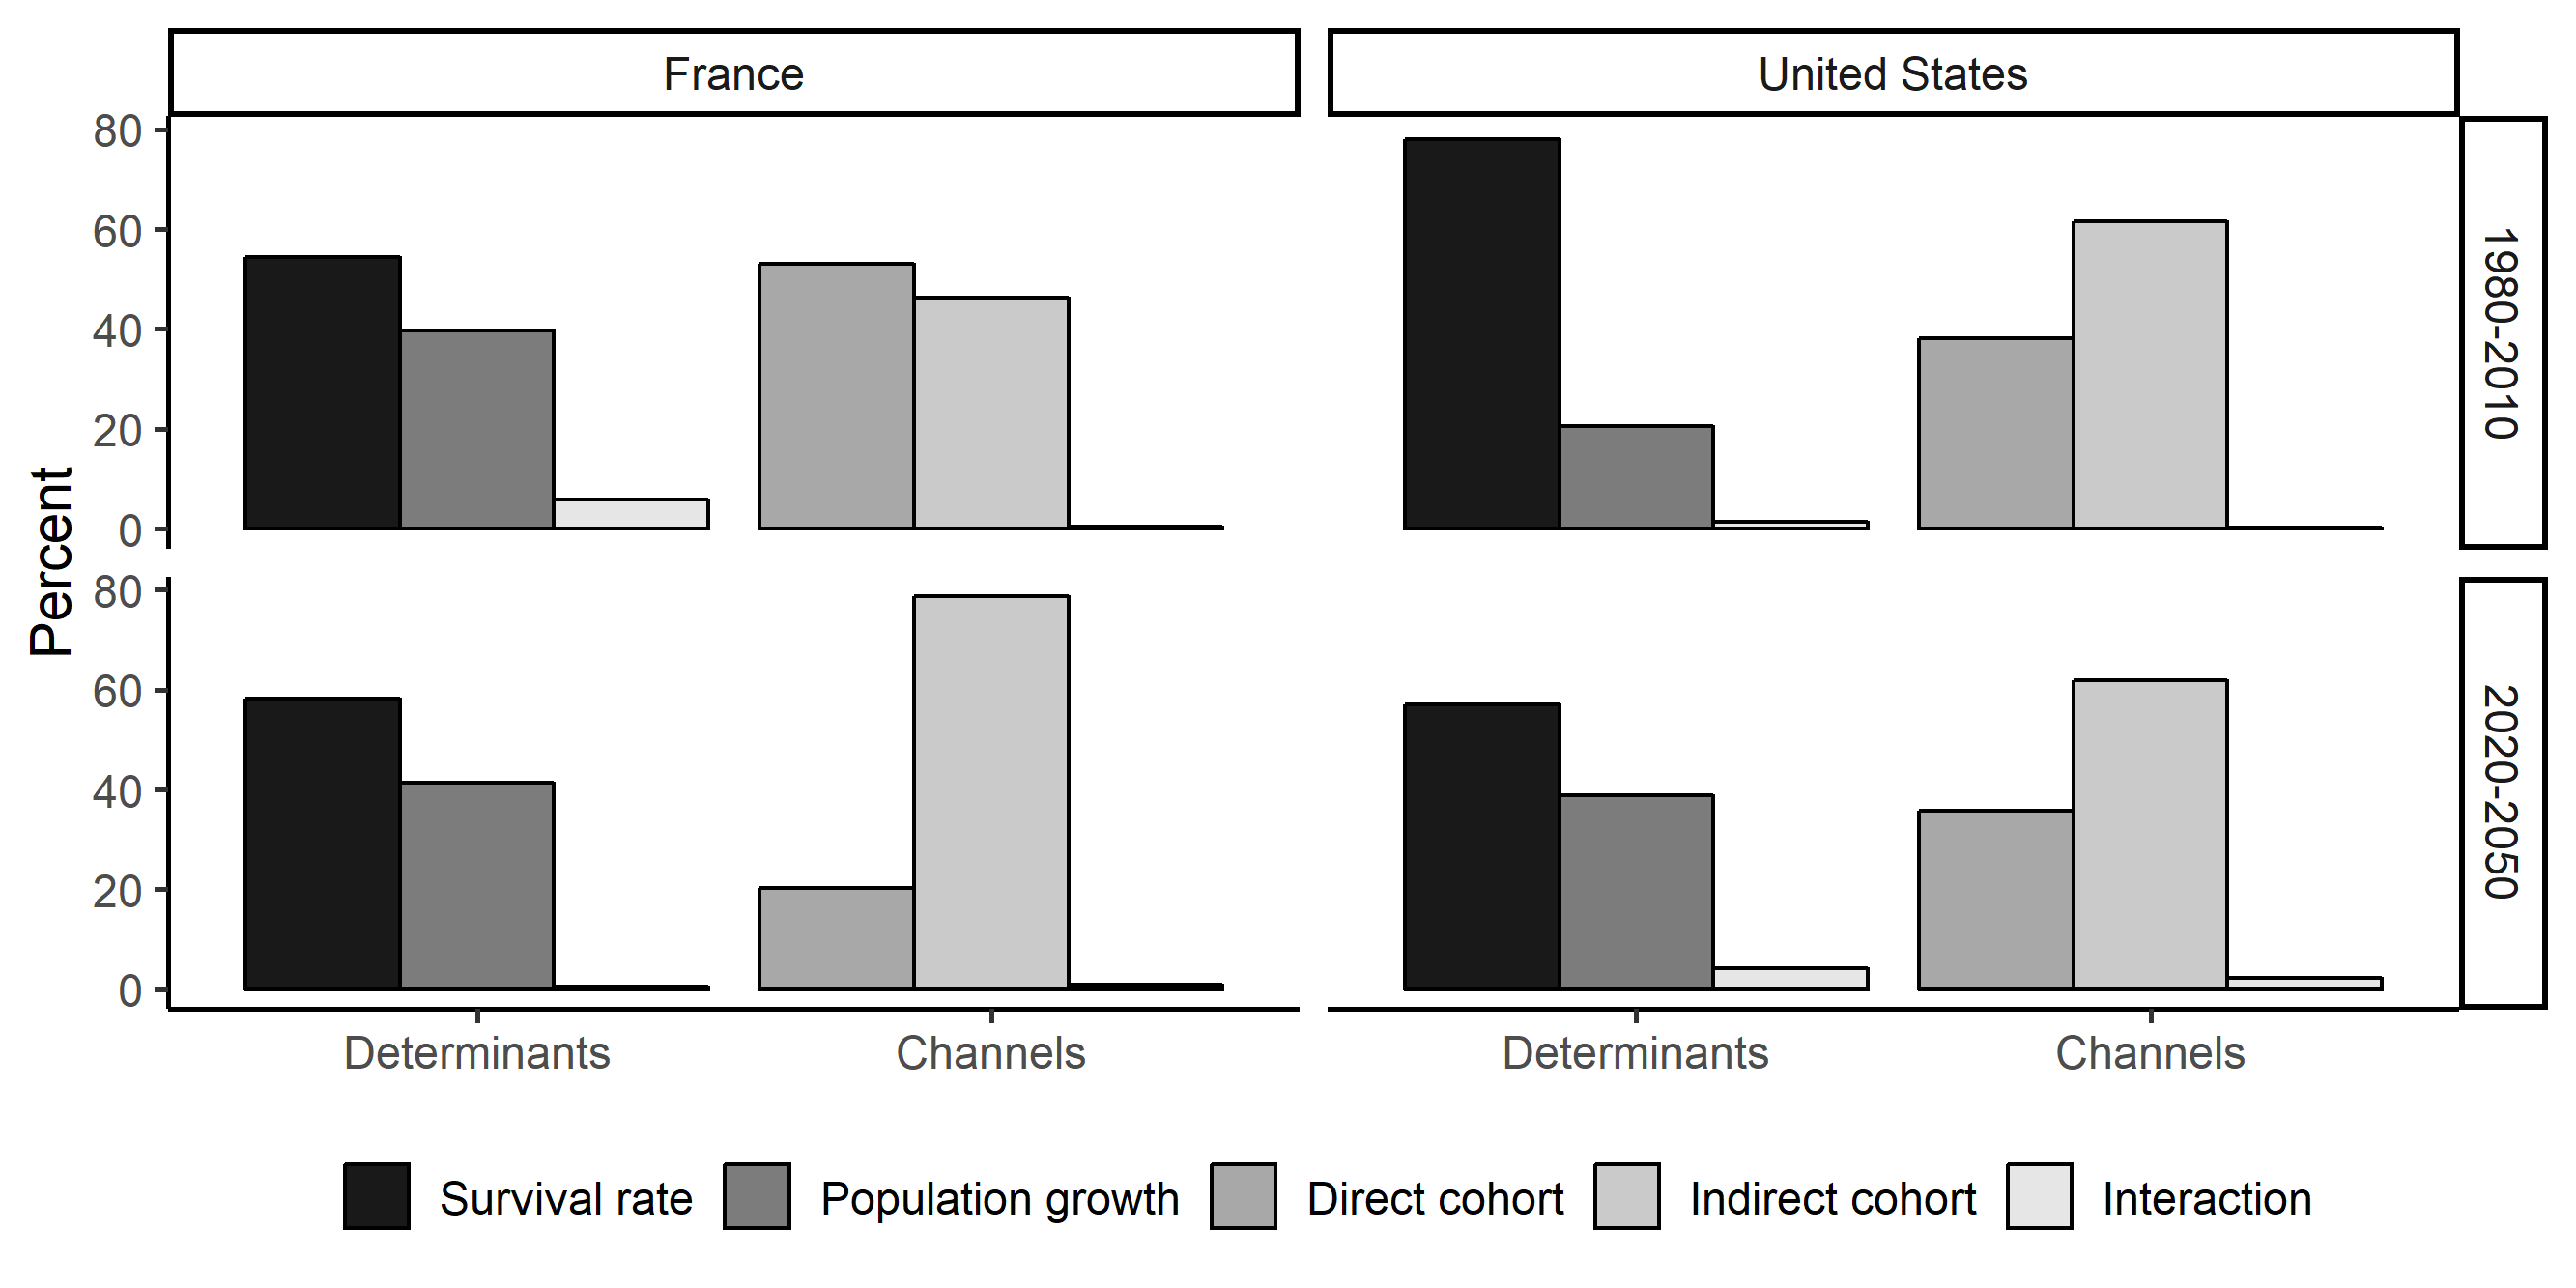
\includegraphics[width=1\linewidth]{../result/decomposition/decomp_country_period.png}
	\caption{Aging-effect decomposition by periods and countries}
	\label{fig:decomp_country_period}
	%	\vspace{.5ex}
	%	\hrule
	%	\vspace{-4ex}
	%	\justify\singlespacing\footnotesize 
\end{figure}
Both countries have almost similar patterns. The main determinant of the aging phenomenon is the survival rate. On average, it explains 54.5\% for France and 78.1\% for the United-States of the impact on the labor share over the period 1980-2010. This decomposition persists thereafter. However, the channel decomposition does not. Between 1980 and 2010, demographic dynamics affect the labor share mainly through the direct channel in France. While the indirect one is dominant in the United-States. On average, the share explained by the direct cohort effect is about 53.1\% for France and 38.2\% for the United-States. However, over the next period, the direct cohort effect is not the dominant channel anymore in France. It falls down to 20.3\%. It suggests that the indirect cohort effect becomes the main carrier of the demographic dynamics on the labor share. While it remains relatively stable in the United-States around 35.7\%.



